
\chapter{Narzędzie i oprogramowanie wykorzystane na potrzeby realizacji tematu}


\section{Biblioteka \protect\textit{Corpus2}}
Biblioteka \emph{Corpus2} \cite{corpus2_web} to zestaw struktur danych i funkcji do przetwarzania korpusów oznaczonych morfosyntaktycznie, z tagsetem pozycyjnym. 
Umożliwia ona wczytywanie i zapisywanie danych do różnych formatów danych takich jak \emph{XCES}, jego rozszerzeniem \emph{CCL} \cite{ccl_web} czy formatów tekstowo-tabelarycznych, takich jak \emph{IOB-Chan} \cite{iob_chan_web}.
Opcjonalnie biblioteka wspiera także pracę, wczytywanie danych, z binarnym i zindeksowanym formatem \emph{Poliqarp} \cite{korpus_ipi_pan} autorstwa pracowników Instytutu Podstaw Informatyki Polskiej Akademii Nauk, a opracowanym w celu przechowywania korpusów tekstowych.
Warto nadmienić, że biblioteka \emph{Corpus2} wspiera także wiele innych formatów plików.

\par 
Biblioteka została zaimplementowana w Instytucie Informatyki Politechniki Wrocławskiej w języku \emph{C++}, ale powstały także skrypty w języku Python, opakowania, umożliwiające pracę z tą biblioteką z wykorzystaniem tego właśnie języka skryptowego.
Dodatkowo narzędzie jest dostępne nieodpłatnie na licencji \emph{GNU LGPL 3.0} lub w przypadku wykorzystania formatu \emph{Poliqarp} na licencji GNU GPL 3.0 \cite{corpus2_web}.

\par
\emph{Corpus2} został wykorzystany w badaniach na potrzeby niniejszej pracy do wczytywania oznaczonych korpusów tekstowych z formatów \emph{IOB-Chan}, \emph{CCL}, a także \emph{Poliqarp}, a także do konwersji pomiędzy nimi.
Ponadto inne narzędzia wykorzystane w tej pracy także wykorzystują funkcjonalność tej biblioteki.


\section{Tagery \protect\textit{WCRFT} i \protect\textit{WCRFT2}}
Nazwa \emph{WCRFT} \cite{wcrft_web} jest akronimem powstałym od słów \emph{Wrocław Conditional Random Fields Tagger} - wrocławskie narzędzie tagujące oparte o model matematyczny \emph{Conditional Random Field}.
\emph{WCRFT} został zaimplementowany z myślą o oznaczaniu tekstów języków fleksyjnych, zwłaszcza słowiańskich, a szczególnie języka polskiego.

\par
Tager napisano w języku Python, z wykorzystaniem gotowej implementacji \emph{CRF} o nazwie \emph{CRF++}, która to napisana została w języku \emph{C++} \cite{wcrft}.
Narzędzie \emph{WCRFT} było implementowane głównie przez Adama Radziszewskiego.

\par
\emph{WCRFT2} natomiast jest następcą tagera \emph{WCRFT}.
Został on napisany całkowicie w języku \emph{C++} -- zostało dokonane portowanie kodu z języka Python do języka \emph{C++}.
Taki zabieg pozwolił na usunięcie zależności związanych z językiem skryptowym, znaczne przyspiesznie tagera (trzykrotne), a także usprawnił i ułatwił proces budowy narzędzia.
Zaznaczyć trzeba, że po wykonaniu konwersji pomiędzy językami zachowano kompatybilność modeli z poprzednią wersją tagera, a wyniki dla obu wersji są takie same.
Ta wersja jest teraz zalecaną do użycia, a poprzednia nie jest już wspierana.

\par
Narzędzie to, w celach badawczych wyszczególnionych w tej pracy, zostało wykorzystane do oznaczenia morfosyntaktycznego słów z zebranych tekstów języka polskiego, które następnie zostały wykorzystane w procesie badania sposobów ekstrakcji kolokacji.
Do wykonania prac wykorzystany został nowy, gotowy model dla tagera udostępniony przez grupę G4.19.

\section{Formalizm \protect\textit{WCCL}}
\subsection{Wyjaśnienie terminu}
\emph{WCCL (Wrocław Corpus Constraint Language)} \cite{wccl_web} jest formalizmem, językiem ograniczeń i narzędziem pozwalającym tworzyć wyrażenia funkcyjne, które można wykorzystać jako cechy (kluczowe informacje), dla wielu algorytmów przetwarzania języka naturalnego i maszynowego uczenia \cite{wccl}. 
Wyrażenia \emph{WCCL} działają na tekście uprzednio oznakowanym morfosyntaktycznie, na przykład za pomocą narzędzia wspomnianego we wcześniejszej części tej pracy -- tagera \emph{WCRFT2}. 
Chociaż formalizm ten był konstruowany z myślą o pracy z językiem polskim, według autorów powinien on także móc być użyty do pracy z innymi językami fleksyjnymi. 
Ograniczeniami mogą być jednak przyjęta tekstowa reprezentacja tagów oraz formaty oznakowanych korpusów, na których miałyby pracować wyrażenia \emph{WCCL} \cite[str. 1]{wccl}.

\par
Omawiany język ograniczeń został zaimplementowany w języku \emph{C++} w postaci bibliotek wykorzystujących \emph{Corpus2} oraz system \emph{MACA (Morphological Analysis Converter and Aggregator)}. 
Dodatkowo napisane zostały także skrypty w języku Python opakowujące funkcjonalność \emph{WCCL} i umożliwiające prace z poziomu języka skryptowego, bez konieczności zaznajomienia się z językiem natywnym, w jakim formalizm ten został zaimplementowany. 
Dzięki temu tworzenie narzędzi i praca z \emph{WCCL} może być szybsza i prostsza \cite[str. 3]{wccl}.

\par
Formalizm \emph{WCCL} został wykorzystany w badaniach z poziomu języka \emph{C++}, bez użycia opakowań, i posłuży głównie do filtrowania kandydatów na jednostki wielowyrazowe na podstawie weryfikacji, jakimi częściami mowy są składowe wyrażenia wielowyrazowego oraz w oparciu o inne cechy, takie jak przykładowo uzgodnienie rzeczownika z przymiotnikiem.
Autor niniejszej pracy zajął się badaniami nad kolokacjami w języku polskim, co rozwiązało ewentualne problemy mogące się pojawić przy pracy z innymi językami fleksyjnymi.

\subsection{Przykładowe wyrażenie}
Przykładowy, prosty operator \emph{WCCL} zbliżony swoją składnią do jednego z operatorów stosowanych w badaniach przeprowadzonych przez autora tej pracy zamieszczono poniżej. 

\begin{lstlisting}[frame=single, tabsize=2, language=Python, caption=Przykładowe wyrażenie w języku \emph{WCCL}, captionpos=b, breaklines=true, basicstyle=\scriptsize]
@b:"SubstAdjOrSubstSubst"
(
	or
	(
		and
		(
			inter(class[0], {subst}),
			inter(class[1], {adj, subst}),
		
			setvar($Case, 0)
		),
		and
		(
			inter(class[1], {subst}),
			inter(class[0], {adj, subst}),
		
			setvar($Case, 1)
		)
	)
)
\end{lstlisting}

Powyższy listing prezentuje kod wyrażenia w języku \emph{WCCL}.
Składa się on z dwóch części - nagłówka i ciała.
Istotną informacją jest fakt, że operator \emph{WCCL} jest kontekstowy, wywoływany jest dla konkretnego miejsca w korpusie, jakiegoś wyrazu w nim zawartego.
Wyraz ten nazwijmy \emph{początkiem kontekstu operatora}.

\par
Nagłówek zawiera dwie informacje o wyrażeniu.
Pierwsza z nich, \emph{@b}, to typ zwracany przez ten operator na podstawie wykonania instrukcji zawartych w jego ciele. 
Druga informacja to nazwa wyrażenia znajdująca się po dwukropku, tutaj będzie to \emph{SubstAdjOrSubstSubst}.
Powyższy kod zwróci jedną z dwóch wartości logicznych - \emph{True} lub \emph{False}.
Inne typy, które mogą zwracać operatory \emph{WCCL} to \emph{Position}, \emph{Set of strings} oraz \emph{Tagset symbol set}.
Pierwszy z nich to wartość całkowita - odpowiednik typu \emph{int} w języku \emph{C++}, drugi typ jest rozumiany jako zbiór ciągów znaków tekstowych, a trzeci to zestaw symboli używanego tagsetu.

\par
Przed opisem ciała powyższego przykładowego operatora należy wyjaśnić funkcje w nim użyte.
Pierwsze dwie z nich są intuicyjne - funkcja \emph{or} i \emph{and}.
Obie z nich zachowują się jak funkcje logiczne o tych samych nazwach anglojęzycznych, a argumenty dla nich są oddzielone przecinkiem tak samo jak w każdej funkcji języka \emph{WCCL}.
Funkcja \emph{setvar} ustawia wartość zmiennej o nazwie podanej w pierwszym argumencie na wartość zadaną parametrem drugim.
Natomiast funkcja \emph{inter} sprawdza przecięcie zbiorów zadanych jej argumentami i zwraca \emph{True} jeśli moc przecięcia jest niezerowa.
Kluczowa w tym wyrażeniu jest także funkcja \emph{class} przyjmująca tylko jeden argument typu całkowitego.
Funkcja ta zwróci klasę gramatyczną słowa oddalonego o zadaną argumentem liczbę wyrazów od \emph{początku kontekstu} tego wyrażenia.
Przykładowo przyjmijmy, że jakiś operator wywołuje kolejno funkcje \emph{class[-1]}, \emph{class[0]} i \emph{class[1]} na poniższym zdaniu, gdzie słowo będące \emph{początkiem kontekstu operatora} zostało oznaczone pogrubioną czcionką:
\begin{center}
Długie, ciężkie \textbf{spodnie} jeszcze się suszą.
\end{center}
Pierwsza funkcja z argumentem równym minus jeden zwróci klasę gramatyczną słowa \emph{ciężkie} czyli przymiotnik, druga klasę wyrazu będącego początkiem kontekstu operatora - \emph{spodnie}, czyli rzeczownik, natomiast wynikiem działania trzeciej dla wyrazu \emph{jeszcze} będzie partykuła.

\par
Ciało powyższego wyrażenia \emph{WCCL} składa się z pojedynczego bloku - funkcji \emph{or}, sprawdzającej czy którykolwiek z dwóch bloków wewnętrznych \emph{and} zwróci wartość \emph{True} i jeśli tak to \emph{or} także zwróci \emph{True} jako wartość testu wykonanego przez ten operator.
Oba wewnętrzne bloki \emph{and} wykonują podobny test na dwóch kolejnych wyrazach z korpusu poczynając od \emph{początku kontekstu} wywołania wyrażenia.
Pierwszy blok \emph{and} sprawdza, czy klasa gramatyczna słowa, dla którego operator został wywołany, jest rzeczownikiem (\emph{subst}), a wyraz kolejny odpowiednio przymiotnikiem (\emph{adj}) lub też rzeczownikiem.
Jeśli obie funkcje \emph{inter} zwrócą \emph{True} to ustawiana jest zmienna, która następnie może zostać odczytana w kodzie programu, który ten operator wywołał.
W przypadku omawianego operatora zmienna \emph{Case} będzie równa zero lub jeden w zależności od tego, która z funkcji \emph{and} zwróci wartość \emph{prawda}.
Może też być niezdefiniowana jeśli obie funkcje \emph{and} zwrócą wartość \emph{fałsz}.
Zabieg taki pozwalać może przykładowo na określenie kolejności wyrazów, w jakiej wystąpiły w korpusie w celu odczytania tej informacji w programie.
Drugi blok \emph{and} zachowuje się analogicznie do pierwszego - sprawdza ten sam warunek, ale dla wyrazów ułożonych w odwrotnej kolejności.

\par
Więcej informacji o wyrażeniach języka \emph{WCCL} można pozyskać zapoznając się z pracą Adama Radziszewskiego, Adama Wardyńskiego i Tomasza Śniatowskiego \cite{wccl}.

\section{Słowosieć}
\emph{Słowosieć} \cite{slowosiec} jest polskim, pierwszym co wielkości na świecie \emph{Wordnetem}, utworzonym i nieustannie rozwijanym przez Grupę Technologii Językowych Politechniki Wrocławskiej G4.19 w ramach projektów \emph{Clarin}, \emph{Synat} oraz \emph{Nekst} przy wsparciu uczelni oraz Ministerstwa Nauki i Szkolnictwa Wyższego.

\par
Aktualna wersja \emph{Słowosieci} jest dostępna na darmowej licencji i zawiera 155 tysięcy słów, 227 tysięcy znaczeń oraz pół miliona relacji, jednak jest także szybko rozwijana przez zespół pracowników, zatem powyższe wartości mogą ulec znacznej zmianie w najbliższym wydaniu nowej wersji tego polskiego \emph{Wordnetu}.
Zawiera ona także 123 tysięcy haseł polsko-angielskich, pozyskanych z \emph{Princeton Wordnet 3.1} \footnote{Informacje ustne od Dr Macieja Piaseckiego -- koordynatora projektu.}.
Dokładniejsze statystyki i więcej informacji znaleźć można na stronie internetowej projektu \cite{slowosiec}.
% Dostępnych jest także wiele publikacji traktujących o \emph{Słowosieci}, spośród których warto wspomnieć o .
% Dodatkowo strona internetowa \emph{Słowosieci}\cite{slowosiec} zawiera spis dostępnych publikacji traktujących o niej.
% Znaleźć tam można także dokładne statystyki, interfejs webowy oraz inne informacji tym o projekcie.

\par
Baza danych polskiego \emph{Wordnetu} wykorzystywana była w celu pozyskania wzorcowych wyrażeń wielowyrazowych.

\section{SuperMatrix}
\emph{SuperMatrix} \cite{supermatrix} to system do budowy modeli z zakresu semantyki dystrybucyjnej \footnote{Informacje ustne od Dr Macieja Piaseckiego.}. 
Pakiet wielu narzędzi zaimplementowanych w języku \emph{C++}, z założenia przystosowany do wykonywania różnych operacji na dwuelementowych obiektach, takich jak przykładowo bi-gramy. 
Narzędzie to oferuje szereg funkcji, programów i gotowych algorytmów, takich jak obliczanie wartości asocjacji z wykorzystaniem wielu miar (ponad osiemdziesięciu), wyliczanie wartości funkcji podobieństwa wierszy względem siebie, filtrowanie danych, transformacje, dzielenie macierzy, ich łącznie i inne.
Zawiera programy oraz skrypty umożliwiające budowanie krotek dwuelementowych i macierzy na kilka sposobów, na podstawie danych z korpusów tekstowych oznaczonych morfosyntaktycznie.
Dla wygody i przyspieszenia pracy napisane zostały także opakowania w języku \emph{Python}, umożliwiające używanie bibliotek i narzędzi z pakietu \emph{SuperMatrix} z poziomu tego języka skryptowego.

\par
Dużą zaletą omawianego narzędzia jest fakt, że było ono z powodzeniem wielokrotnie wykorzystywane, oraz że mimo dużej funkcjonalności jest ono dostępne na darmowej licencji i można je nieodpłatnie pobrać z sieci Internet.

\par
Istotne jest, że dane składowane są w postaci macierzy dwuwymiarowej (podstawowego formatu danych dla narzędzi w tym pakiecie), co jest ograniczeniem i problemem w przypadku zamiaru pracy z kolokacjami dłuższymi niż dwuelementowe. 
Jednak zarówno to ograniczenie jak i fakt, że \emph{SuperMatrix} nie był projektowany do pracy z kolokacjami, nie jest problemem dla prowadzenia badań nad wyrażeniami dwuelementowymi. 
Wystarczy jedynie przygotować dane w odpowiedni sposób i wedle potrzeby, a następnie wykorzystać możliwości zawarte w pakiecie narzędzi.

\par
Pierwsze badania na potrzeby tej pracy wykonywane były z wykorzystaniem właśnie tego pakietu narzędzi ze względu na liczność zaimplementowanych miar asocjacji, które można było zbadać bez konieczności przystosowywania narzędzia, implementacji nowych modułów pakietu, kolejnych programów czy całej aplikacji specjalnie do tego celu.
Badania te pozwoliły przetestować dziesiątki miar i ocenić, którymi z nich warto zająć się przy dalszej pracy z jednostkami wielowyrazowymi dłuższymi niż dwuelementowe.
Pierwsze wyniki nadały pewien kierunek dla prowadzania dalszych prac w temacie wyrażeń wielowyrazowych.

\section{\protect\textit{MWeXtractor}}
Pakiet narzędzi \emph{SuperMatrix} z założenia miał być wykorzystywany do pracy z parami elementów, z których jeden jest reprezentowany danymi zawartymi w wierszu, a drugi w kolumnie macierzy.
Cecha ta jest swoistego rodzaju ograniczeniem i problemem być może uniemożliwiającym, a na pewno bardzo utrudniającym prowadzenie badań obiektów, składających się z trzech lub większej liczby elementów.
Sposób przechowywania danych i ich wykorzystania musiałby zostać przygotowany do składowania w formacie pakietu \emph{SuperMatrix}, czyli dwuwymiarowej macierzy, co znacząco utrudniałoby wykonanie zadania.
Dodatkowo zabieg ten wydaje się niewłaściwy koncepcyjnie.
To format danych powinien być dopasowany do składowania określonych danych, a nie dane upakowane na siłę w taki sposób, aby zmieściły się w narzuconym formacie, nieprzygotowanym do przechowywania informacji tego rodzaju.
Sam sposób przechowywania danych był jednak tylko jednym z problemów.
Praktycznie wszystkie narzędzia pakietu \emph{SuperMatrix} zostały przygotowane do pracy z obiektami dwuelementowymi.
Fakt ten oznacza, że wykorzystanie omawianego narzędzia byłoby niewielką wartością dodaną w prowadzeniu badań, ponieważ dużą część funkcjonalności trzeba byłoby zaimplementować od nowa, mając na uwadze ograniczenia i koncepcje wprowadzone na potrzeby realizacji projektu \emph{SuperMatrix}.
Reimplementacja metod wymagana byłaby także ze względu na wspomnianą wcześniej konieczność upakowania danych N-elementowych do postaci dwuelementowej.
Mogłoby to doprowadzić do poświęcenia dużej ilości czasu i uwagi na zaplanowanie, dostosowanie, implementację i integrację nowych fragmentów oprogramowania \emph{SuperMatrix} zamiast wykorzystania tych zasobów do realizacji faktycznego zadania, będącego celem niniejszej pracy.

\par
Omówione problemy były jednymi z głównych przyczyn opracowania nowego narzędzia, niezależnego od pakietu \emph{SuperMatrix}, specjalizowanego pod kątem prowadzania badań dotyczących wyrażeń wielowyrazowych.
Narzędzie \emph{MWeXtractor} utworzone przez autora tej pracy jest biblioteką programistyczną oraz pakietem struktur danych, programów, skryptów i niewielkiej ilości danych.
Posłużyło ono do prowadzenia badań nad kolokacjami, których wyniki zostały zamieszczone w dalszej części niniejszej pracy.

\par
Większość oprogramowania, a w szczególności jego główne funkcjonalności zostały zaimplementowane w języku \emph{C++} w celu osiągnięcia jak największej wydajności pamięciowej odnośnie składowania danych oraz obliczeniowej narzędzi i algorytmów.
Wykorzystany standard tego języka to \emph{C++11}.
Język skryptowy \emph{Python} został wykorzystany do utworzenia części oprogramowania pomocniczego - skryptów.
Oprogramowanie związane z algorytmem genetycznym pochodzi z kodów zaimplementowanych przez Łukasza Kłyka \cite{klyk}, a zostało dostosowane przez autora niniejszej pracy do współpracy z omawianym pakietem narzędzi \emph{MWeXtractor}.


\subsection{Przykładowe schematy użytkowania narzędzia}
Dwie typowe ścieżki przetwarzania umożliwione przez oprogramowanie \emph{MWeXtractor} zostały opisane w dalszej części pracy.
Pierwsza z nich jest związana z badaniem jakości funkcji asocjacyjnych i klasyfikatorów, a druga służy do ekstrakcji kolokacji z korpusów tekstowych.

\subsection{Schemat procesu badania metod ekstrakcji kolokacji}
Schemat \ref{user_processing_scheme_research} prezentuje pierwszą z dwóch typowych ścieżek przetwarzania, odpowiedzialną za badania metod ekstrakcji wyrażeń wielowyrazowych.

\begin{figure}[h!]
\centering
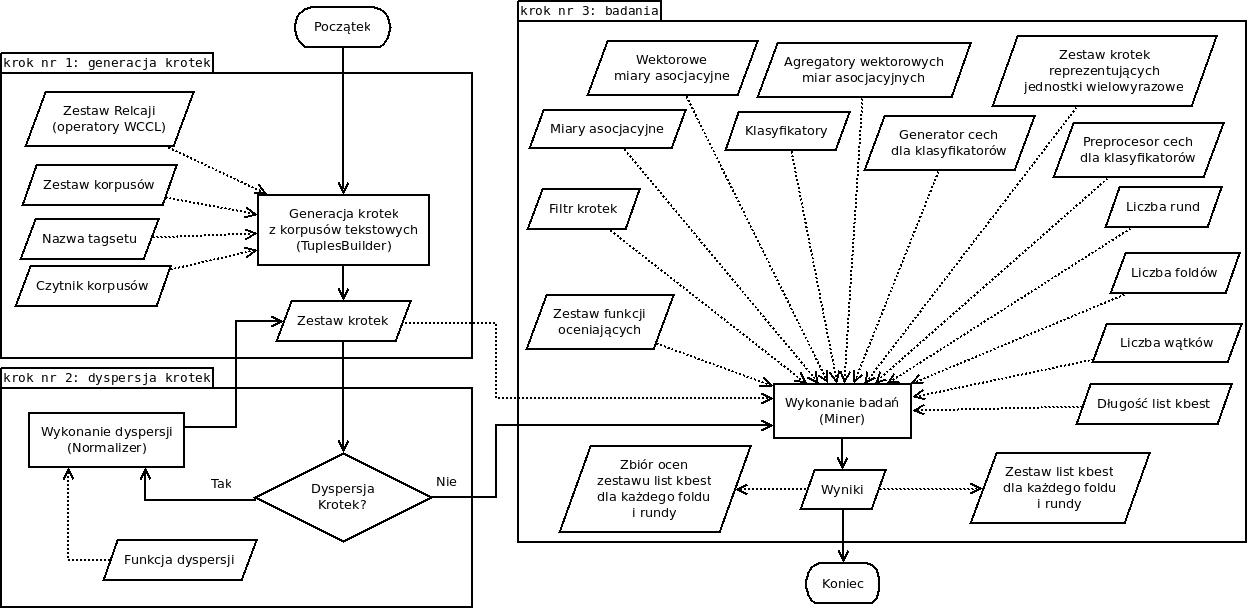
\includegraphics[width=\textwidth]{charts/user_processing_scheme_research.jpg}
\caption [Przykładowy schemat procesu badania jakości rankerów]{Schemat jednego z typowych procesów użytkowania oprogramowania \emph{MWeXtractor} -- badania jakości generowanych przez rankery kolokacji.}
\label{user_processing_scheme_research}
\end{figure}

\par
\noindent\textbf{Krok numer 1: generacja krotek}
\par
Najpierw należy przygotować listę korpusów, z których mają zostać wydobyte dane do przeprowadzenia badań nad metodami ekstrakcji wyrażeń wielowyrazowych.
Należy podać typ czytnika korpusów oraz tagset jakim dane tekstowe zostały opisane.
Następnie zdefiniować zestaw relacji -- operatorów zapisanych w języku \emph{WCCL}, które specyfikują jakich kandydatów na wyrażenia wielowyrazowe należy wyszukiwać w badanych korpusach tekstowych.
Dzięki nim można ograniczyć zestaw kandydatów, nad którymi chce się prowadzić badania.
Jeśli użytkownik jest zainteresowany wszystkimi możliwymi do utworzenia n-gramami może przykładowo wykorzystać do tego celu operator \emph{WCCL} generujący wszystkie możliwe kombinacje n-elementowe.
Zaznaczyć trzeba, że wydobywani kandydaci na kolokacje nie muszą posiadać cechy ciągłości, ich szyk może być zmienny, a wszystko zależy od tego jak zostaną przygotowane relacje.
Tak przygotowany zestaw danych i parametrów należy następnie podać jako argumenty dla programu \emph{TuplesBuilder}, który na ich podstawie przygotuje skład krotek -- podstawową strukturę danych dla oprogramowania \emph{MWeXtractor} składującą krotki.

\par
\noindent\textbf{Krok numer 2: dyspersja krotek}
\par
Drugi krok tego schematu przetwarzania jest opcjonalny i dotyczy modyfikacji informacji o zebranych krotkach -- ich częstości będących kluczowym elementem związanym z późniejszą oceną kandydatów na kolokacje.
Do tego celu wykorzystana może zostać jedna z funkcji dyspersji zaimplementowana w tym celu.
Funkcje te zostaną opisane w dalszej części pracy.
Zależnie od wybranej metody dyspersji pod uwagę brane są różne statystyki związane z krotkami, przykładowo będą to częstości danych krotek, liczba krotek w danym korpusie czy informacja o tym, w ilu korpusach dana krotka została odnaleziona.
Mówiąc inaczej, miara dyspersji ma za zadanie zmienić rozkład częstości krotek w składzie\footnote{Skład krotek to podstawowa struktura do przechowywania danych statystycznych wydobytych z korpusów tekstowych, przechowuje między innymi rodzaje i częstości kandydatów na kolokacje. Jej dokładniejszy opis został zamieszczony w dalszej części niniejszego rozdziału, aby nie wprowadzać szczegółów mogących utrudnić zrozumienie ogólnej koncepcji działania systemu.} promując instancje ciekawe -- mniej typowe.
\par
Jedna z zaimplementowanych funkcji dyspersji\footnote{Funkcje dyspersji zostaną opisane w dalszej części niniejszego rozdziału.} -- \emph{Lynes D3} \cite{dispersions}, bazuje na mierze $ Chi^{2} $, a tym samym potrzebne są jej pewne dane statystyczne.
Jeśli ta miara ma zostać wykorzystana do dyspersji krotek, to trzeba jej owe dane statystyczne przygotować.
Sposób generacji tych informacji został opisany w trzecim kroku kolejnego z przykładowych schematów przetwarzania.
Zaznaczyć jednak trzeba, że miara \emph{Lynes D3} to wyjątek.

\par
\noindent\textbf{Krok numer 3: badania}
\par
Niniejszy krok jest krokiem finalnym ścieżki przetwarzania.
Polega on na wykonaniu r-rundowej, f-foldowej walidacji krzyżowej dla danego zbioru danych, z wykorzystaniem określonych miar asocjacyjnych i klasyfikatorów.
Oprogramowanie przeznaczone do tego celu zostało nazwane \emph{Miner}.
Wyniki wygenerowane przez ten program zostają poddane ocenie przez użytkownika narzędzi \emph{MWeXtractor}. 
Do łączenia dużych zestawów wyników przygotowany został skrypt w języku \emph{Python} uśredniający wyniki dla wszystkich foldów z każdej z rund, dla poszczególnych funkcji rankingowych z osobna.
Pozwala to na szybkie wygenerowanie zbiorczych wyników i na utworzenie wykresów prezentujących jakości rezultatów zastosowanych metod wydobycia według określonych miar.
\par
Parametry programu \emph{Miner} zostały wymienione i opisane w tabeli \ref{miner_parameters}.

\begin{table}[h!]
\centering
\begin{tabular}{l | l | p{0.6\linewidth}}
	\toprule 
	\textbf{Nazwa} & \textbf{Typ} & \textbf{Opis} \\
	\midrule 
	Skład krotek & nazwa folderu & ścieżka do folderu ze składem krotek \\ 
	\hline
	Wyjście programu & nazwa folderu & ścieżka do folderu, w którym zostaną zamieszczone wyniki\\ 
	\hline
	Miary asocjacji & ciągi tekstowe & parametr wielokrotny, tekst reprezentujący funkcje asocjacyjną, którą program ma wykorzystać\\ 
	\hline
	Miary wektorowe & ciągi tekstowe & parametr wielokrotny, tekst reprezentujący wektorową miarę asocjacyjną, którą program ma wykorzystać\\ 
	\hline
	Agregatory & ciągi tekstowe & parametr wielokrotny, tekst reprezentujący funkcję agregującą wyniki miar wektorowych, po jednej funkcji dla każdej z nich\\
	\hline
	Klasyfikatory & ciągi tekstowe & parametr wielokrotny, tekst reprezentujący klasyfikator, który program ma wykorzystać\\ 
	\hline
	Generator cech & ciąg tekstowy & wektorowa miara asocjacyjna, która zostanie wykorzystana jako generator cech dla klasyfikatorów\\ 
	\hline
	Preprocesor cech & ciąg tekstowy & parametr opcjonalny, tekst reprezentujący funkcję, która ma zostać wykorzystana do normalizacji cech\\ 
	\hline
	Zestaw JW & nazwa pliku & plik zawierający w każdej linii ciąg wyrazów oddzielonych spacjami, reprezentujący wyrażenie wielowyrazowe\\ 
	\hline
	Funkcje oceny & ciągi tekstowe & parametr wielokrotny, tekst reprezentujący funkcję oceny, którą program ma wykorzystać\\ 
	\hline
	Filtr krotek & ciąg tekstowy & tekst reprezentujący filtr, który program ma wykorzystać do wyznaczenia zestawu krotek, z których ma korzystać i, dla których wygenerować dane\\ 
	\hline
	Liczba wątków & liczba całkowita & maksymalna liczba wątków do wykorzystania przez program\\ 
	\hline
	Liczba rund & liczba całkowita & liczba rund walidacji krzyżowej\\ 
	\hline
	Liczba foldów & liczba całkowita & liczba foldów dla każdej walidacji krzyżowej\\
	\bottomrule
\end{tabular}
\caption[Parametry programu \emph{Miner}]{Tabela zawiera nazwy, typy oraz opisy parametrów wykorzystywanych przez program \emph{Miner}}
\label{miner_parameters}
\end{table}

\par
Wspomniany zbiór wyników jest obszerny, podzielony na pliki, których są dwa rodzaje -- pliki z listami k-najlepszych kandydatów na wyrażenia wielowyrazowe, oraz pliki z ocenami tych list.
Liczba wygenerowanych plików rankingowych jest równa \( ((A + V + C) * R * F) \), gdzie \emph{A}, \emph{V} oraz \emph{C} oznaczają kolejno liczbę wykorzystanych funkcji asocjacyjnych, wektorowych miar asocjacyjnych oraz klasyfikatorów, natomiast \emph{R} i \emph{F} to kolejno liczba rund i foldów walidacji krzyżowej.
Dodatkowo dla każdego pliku z rankingiem wygenerowanych zostaje \emph{Q} plików oceny tego rankingu, gdzie \emph{Q} jest liczbą wykorzystanych funkcji oceny list k-najlepszych.
Wzorzec nazwy pliku z rankingiem jest generowany w sposób następujący: \emph{kbest.nr\_rankera.nr\_rundy.nr\_foldu.csv}, natomiast wzorzec dla plików z wynikami funkcji oceny list k-najlepszych to: \emph{kbest.nr\_rankera.nr\_rundy.nr\_foldu.nr\_funkcji\_oceny.csv}.
Numer rankera\footnote{Ranker to pojęcie wprowadzone przez autora pracy na ogólne określenie metod i algorytmów generujących rankingi pewnych bytów. W przypadku niniejszej pracy i tematyki tutaj poruszanej rankerami są funkcje asocjacyjne, wektorowe miary asocjacyjne oraz klasyfikatory, a zadaniem każdego z nich jest wygenerowanie rankingu kandydatów na kolokacje.} jest z przedziału:
\begin{enumerate}
  \item \texttt{[0     : A         - 1]} -- dla funkcji asocjacyjnych;
  \item \texttt{[A     : A + V     - 1]} -- dla wektorowych miar asocjacyjnych;
  \item \texttt{[A + V : A + V + C - 1]} -- dla klasyfikatorów.
\end{enumerate}

Ze względu na dużą liczbę plików wynikowych zaimplementowany został skrypt wspomniany wcześniej, łączący wyniki poprzez uśrednienie wyników dla każdego foldu z każdej rundy dla poszczególnych funkcji rankingujących z osobna.
Skrypt ten generuje pojedynczy plik z jedną kolumną dla każdego rankera.
Skrypt nazwany został \emph{cv\_quality\_merger.py}, został napisany w języku \emph{Python} i jest częścią pakietu \emph{MWeXtractor}.


\subsection{Schemat procesu ekstrakcji wyrażeń wielowyrazowych}
Schemat \ref{user_processing_scheme_extraction} prezentuje drugą z dwóch typowych ścieżek przetwarzania, odpowiedzialną za ekstrakcje wyrażeń wielowyrazowych bez wykonywania badań.

\begin{figure}[h!]
\centering
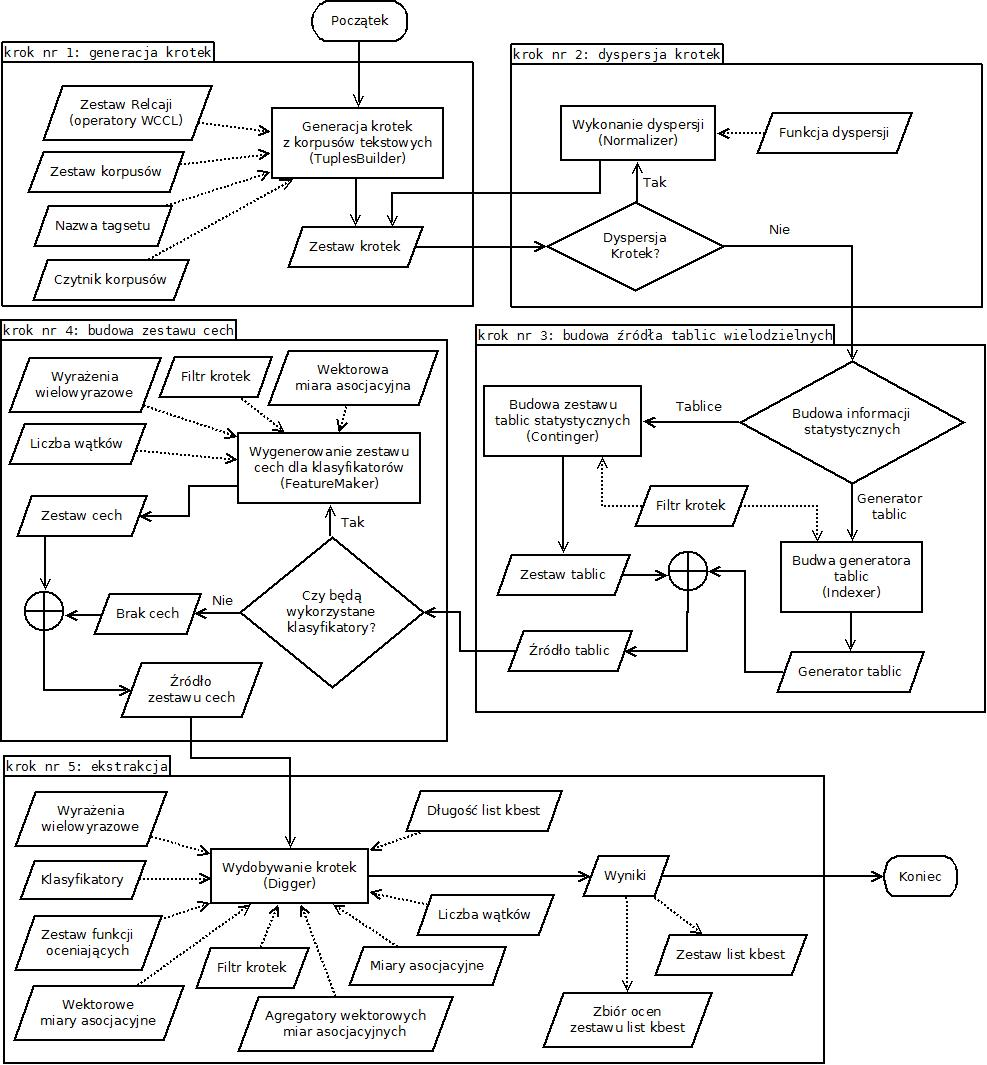
\includegraphics[width=\textwidth]{charts/user_processing_scheme_extraction.jpg}
\caption [Przykładowy schemat procesu wydobywania wyrażeń wielowyrazowych]{Schemat prezentujący jeden z typowych procesów wydobywania wyrażeń wielowyrazowych za pomocą oprogramowania \emph{MWeXtractor}}
\label{user_processing_scheme_extraction}
\end{figure}

\par
\noindent\textbf{Kroki numer 1 i 2}
\par
Oba krotki są takie same jak w przypadku poprzedniego przykładowego schematu przetwarzania -- badania miar asocjacyjnych i klasyfikatorów \footnote{por. rozdz. 4.6.2.}.

\par
\noindent\textbf{Krok numer 3: budowa źródła tablic wielodzielnych}
\par
Wszystkie zaimplementowane miary i klasyfikatory korzystają z informacji zawartych w tablicach wielodzielnych dla krotek. 
Miary korzystają z tych informacji bezpośrednio do obliczania wartości dla kolokacji, a w przypadku klasyfikatorów miary te wykorzystywane są do generowania cech instancji.
Wyjątkiem są miary oparte na szyku, ponieważ nie korzystają z takich informacji.
Krok trzeci polega na utworzeniu jednego z dwóch dostępnych źródeł tablic -- ich generatora lub składu. 
Programy przygotowane do wykonania tego zadania to odpowiednio \emph{Indexer} oraz \emph{Continger}.
Zazwyczaj generator tablic zajmuje znacznie mniej pamięci operacyjnej -- kilkakrotnie mniej niż tablice wielodzielne, ale odwołanie się do tablic jest znacznie wolniejsze niż w przypadku składu tablic, ponieważ generator tworzy je na bieżąco, a skład przechowuje już gotowe tablice.
Zestaw krotek, na podstawie których źródło tablic ma zostać wygenerowane można ograniczyć za pomocą filtrów.
Zabieg taki pozwala na używanie określonego składu krotek do różnych celów, bez konieczności wydobywania kandydatów z korpusów wielokrotnie.
Dodatkowo umożliwia to zbudowanie informacji statystycznych na podstawie innego zestawu krotek niż ten, z którego wyrażenia wielowyrazowe mają być wydobywane.
Jako praktyczny przykład takiego zadania można podać ten, w którym informacja statystyczna budowana jest na podstawie krotek zebranych za pomocą relacji okna, a wydobywanie wyrażeń wielowyrazowych jedynie na podstawie innych relacji, przykładowo o określonych wzorcach strukturalnych.

\par
\noindent\textbf{Krok numer 4: budowanie zestawu cech}
\par
Niniejszy krok jest opcjonalny i może zostać pominięty, jeśli użytkownik nie ma zamiaru korzystać z klasyfikatorów.
Jeżeli jednak użytkownik będzie chciał skorzystać z klasyfikatorów lub wygenerować zestaw cech, z których będzie można korzystać w oprogramowaniu \emph{WEKA}, może do tego celu użyć programu o nazwie \emph{FeatureMaker}.
Zadaniem tego modułu jest wygenerowanie cech dla kandydatów na kolokacje, spośród których mają być w przyszłości wydobyte wyrażenia wielowyrazowe.
Do wykonania tego zadania generator cech wykorzystuje miary asocjacyjne, których wyniki traktowane są jako cechy.
Dopuszczalne jest także wykorzystanie uprzednio wyuczonych klasyfikatorów, przykładowo sieci neuronowych, do generowania cech opisujących kandydatów.
Zestaw kandydatów można ograniczyć za pomocą filtru jeśli nie ma potrzeby wyznaczenia cech dla wszystkich krotek.
\par
Aktualnie jedynym wspieranym formatem pliku wykorzystywanym do zapisu zestawu cech w pamięci nieulotnej, jest \emph{ARFF}.
\par
Tabela \ref{feature_maker_parameters} zawiera opisy parametrów programu \emph{FeatureMaker}.

\begin{table}[h!]
\centering
\begin{tabular}{l | l | p{0.6\linewidth}}
	\toprule 
	\textbf{Nazwa} & \textbf{Typ} & \textbf{Opis} \\
	\midrule 
	Skład krotek & nazwa folderu & ścieżka do folderu ze składem krotek \\ 
	\hline
	Wyjście programu & nazwa pliku & ścieżka do pliku, w którym zostaną zapisane wyniki\\ 
	\hline
	Zestaw JW & nazwa pliku & plik zawierający w każdej linii ciąg wyrazów oddzielonych spacjami, reprezentujący wyrażenie wielowyrazowe, wykorzystany w przypisywaniu klas krotkom\\ 
	\hline
	Generator cech & ciągi tekstowe & tekst reprezentujący wektorową miarę asocjacyjną, którą program ma wykorzystać do generowania cech dla krotek\\ 
	\hline
	Filtr krotek & ciąg tekstowy & tekst reprezentujący filtr, który program ma wykorzystać do wyznaczenia zestawu krotek, dla których wygenerować cechy\\ 
	\hline
	Liczba wątków & liczba całkowita & maksymalna liczba wątków do wykorzystania przez program\\ 
	\bottomrule
\end{tabular}
\caption[Parametry programu \emph{FeatureMaker}]{Tabela zawierająca nazwy, typy oraz opisy parametrów wykorzystywanych przez program \emph{FeatureMaker}}
\label{feature_maker_parameters}
\end{table}

\par
\noindent\textbf{Krok numer 5: ekstrakcja}
\par % TODO: Digger modifications: classifiers + features
Ostatnim krokiem tej ścieżki przetwarzania jest wykorzystanie wcześniej utworzonych danych do ekstrakcji wyrażeń wielowyrazowych z korpusów tekstowych.
Zadanie to może zostać wykonane za pomocą programu \emph{Digger}.
Zestaw parametrów programu jest zbliżony do tych dla narzędzia \emph{Miner}.
W tabeli \ref{digger_parameters} opisane zostały argumenty dla oprogramowania \emph{Digger}.

\begin{table}[h!]
\centering
\begin{tabular}{l | l | p{0.6\linewidth}}
	\toprule 
	\textbf{Nazwa} & \textbf{Typ} & \textbf{Opis} \\
	\midrule 
	Skład krotek & nazwa folderu & ścieżka do folderu ze składem krotek \\ 
	\hline
	Źródło tablic & nazwa pliku & ścieżka do pliku ze składem lub generatorem krotek\\
	\hline
	Wyjście programu & nazwa folderu & ścieżka do folderu, w którym zostaną zamieszczone wyniki\\ 
	\hline
	Miary asocjacji & ciągi tekstowe & parametr wielokrotny, tekst reprezentujący funkcje asocjacyjną, którą program ma wykorzystać\\ 
	\hline
	Miary wektorowe & ciągi tekstowe & parametr wielokrotny, tekst reprezentujący wektorową miarę asocjacyjną, którą program ma wykorzystać\\ 
	\hline
	Agregatory & ciągi tekstowe & parametr wielokrotny, tekst reprezentujący funkcję agregującą wyniki miar wektorowych, po jednej funkcji dla każdej z nich\\
	\hline
	Klasyfikatory & ciągi tekstowe & parametr wielokrotny, tekst reprezentujący klasyfikator, który program ma wykorzystać\\ 
	\hline
	Źródło cech & nazwa pliku & Źródło zestawu cech dla krotek\\ 
	\hline 
	Zestaw JW & nazwa pliku & plik zawierający w każdej linii ciąg wyrazów oddzielonych spacjami, reprezentujący wyrażenie wielowyrazowe\\ 
	\hline
	Funkcje oceny & ciągi tekstowe & parametr wielokrotny, tekst reprezentujący funkcję oceny, którą program ma wykorzystać\\ 
	\hline
	Filtr krotek & ciąg tekstowy & tekst reprezentujący filtr, który program ma wykorzystać do wyznaczenia zestawu krotek, z których ma korzystać i, dla których wygenerować dane\\ 
	\hline
	Liczba wątków & liczba całkowita & maksymalna liczba wątków do wykorzystania przez program\\ 
	\bottomrule
\end{tabular}
\caption[Parametry programu \emph{Digger}]{Tabela zawierająca nazwy, typy oraz opisy parametrów wykorzystywanych przez program \emph{Digger}}
\label{digger_parameters}
\end{table}

Zestaw generowanych wyników jest podobny do tego, który generuje narzędzie \emph{Miner}, ale jest mniejszy, ponieważ nie ma podziału na rundy i foldy ze względu na brak walidacji krzyżowej.
Wzorce nazw dla plików k-najlepszych krotek i plików z ocenami prezentują się teraz następująco: \emph{kbest.nr\_rankera.csv} oraz \emph{quality.nr\_rankera.nr\_funkcji\_oceny.csv}.
Zasada generowania numeru rankera jest taka sama jak w przypadku programu \emph{Miner}.


\subsection{Funkcjonalności dodatkowe}
Pakiet narzędzi \emph{MWeXtractor} posiada też dodatkowe funkcjonalności, z których część została opisana w tym rozdziale.

\par
\noindent\textbf{Program \textit{Cover}}
\par
Program nazwany \emph{Cover} służy do weryfikacji relacji oraz badania przecięcia zbioru wydobytych krotek pomiędzy relacjami -- sprawdzenia, jak wiele z nich zostało przyporządkowanych do więcej niż jednej relacji.
Praktyczne wykorzystanie tego oprogramowania to sprawdzenie pokrycia wzajemnego operatorów \emph{WCCL} zastosowanych do wydobywania krotek z tekstów.
Wynikiem jego działania jest macierz kwadratowa o wymiarze równym liczbie relacji wykorzystanych w procesie tworzenia \emph{składu krotek}, gdzie każdy z wierszy i każda z kolumn mają przypisaną do siebie określoną nazwę operatora \emph{WCCL}.
Liczby całkowite zapisane na przecięciu wierszy z kolumnami informują, ile różnych krotek zostało przypisanych zarówno do relacji będącej etykietą wiersza, jak i kolumny.
Interpretacją liczby na przecięciu wiersza i kolumny -- diagonali, odpowiadającym tej samej relacji jest informacja o tym, ile krotek zostało zakwalifikowanych do tej relacji.
Jeśli w danym wierszu lub kolumnie, poza polem na diagonali macierzy, wystąpi więcej niż jedna wartość większa od zera  oznacza to, że relacje są nierozłączne -- część krotek przyporządkowano do więcej niż jednej relacji.
Należy jednak pamiętać, że narzędzie to nie jest wyrocznią, ponieważ jeśli dla danego zbioru danych okaże się, że relacje są rozłączne, nie oznacza to, że dla innego zbioru, większego czy lepiej oddającego rzeczywistość, sytuacja się powtórzy.
Zbudowana w ten sposób macierz jest symetryczna.
\par
Opisywany tutaj program \emph{Cover} ma także drugie zastosowanie wspomniane we wcześniejszej części tego fragmentu pracy -- badanie przecięcia zbioru krotek ze składu i zestawu zadanego parametrem programu.
Na podstawie zadanego pliku z ciągami wyrazów program bada ile z nich, oraz które konkretnie ciągi zostały odnalezione w \emph{składzie krotek}.
Funkcjonalność ta może posłużyć przykładowo do wyznaczania zbioru krotek pozytywnych, czyli wyrażeń wielowyrazowych, które zostały w tym tekście odnalezione podczas wydobywania kandydatów na kolokacje.
Dodatkowo zakres poszukiwań wśród krotek w składzie można zawęzić za pomocą filtru.
Zabieg taki pozwala na lepsze poznanie zbioru danych.

\par
\noindent\textbf{Wydobywanie form napotkanych}
\par
Program \emph{Digger} umożliwia dodatkowo wydobycie form napotkanych dla krotek z wygenerowanych list k-najlepszych kandydatów na kolokacje.
Jeśli użytkownik jest zainteresowany ekstrakcją form napotkanych to powinien podać cztery dodatkowe parametry dla tego programu, które zostały opisane w tabeli \ref{digger_parameters_orths}.

\begin{table}[h!]
\centering
\begin{tabular}{l | l | p{0.5\linewidth}}
	\toprule 
	\textbf{Nazwa} & \textbf{Typ} & \textbf{Opis} \\
	\midrule 
	Zestaw korpusów & nazwa pliku & ścieżka do pliku zawierającego listę ścieżek do korpusów, po jednej ścieżce w każdej linii pliku \\ 
	\hline
	Operatory WCCL & nazwa pliku & ścieżka do pliku z operatorami języka \emph{WCCL}, które były użyte przy wydobywaniu kandydatów na kolokacje w kroku numer jeden\\ 
	\hline
	Tagset & ciąg znaków & nazwa wykorzystanego tagsetu w korpusach \\
	\hline
	Czytnik & ciąg znaków & nazwa czytnika korpusów\\
	\bottomrule
\end{tabular}
\caption[Parametery dodatkowe programu \emph{Digger}]{Tabela zawierająca nazwy, typy oraz opisy parametrów dodatkowych wykorzystywanych przez program \emph{Digger}.}
\label{digger_parameters_orths}
\end{table}

Wyekstrahowany zestaw form napotkanych dla krotek zostanie zapisany w pojedynczym pliku w formacie \emph{CSV}.
Format pliku jest następujący: najpierw zapisana zostaje reprezentacja krotki z jednej z list k-najlepszych, a część kolejnych linii rozpoczyna się tabulacją i zawiera ciąg wyrazów napotkanych dla tej krotki wraz z jego częstością.
Następnie zapis taki powtarza się dla wszystkich wydobytych krotek, jeśli jest ich więcej, ale bez powtórzeń, jeśli krotki wystąpiły na różnych listach k-najlepszych.
Dodatkowo napisany został skrypt łączący listy k-najlepszych z zestawem wydobytych dla nich form napotkanych i tworzący nowe listy k-najlepszych z zachowaniem przy tym kolejności rankingu.
Skrypt przypisuje również do każdej pozycji zestaw form napotkanych tej krotki wraz z ich częstościami.
Kolejność form napotkanych po łączeniu będzie posortowana malejąco według ich częstości.
Skrypt ten, napisany w języku \emph{Python}, został nazwany \emph{kbest\_orth\_merger.py} i jest częścią pakietu \emph{MWeXtractor}.


\subsection{Format składowania krotek zebranych z korpusów}
Jako format przechowywania danych wykorzystano krotki o różnych długościach\footnote{Długość krotki rozumiana jest jako liczba jej elementów składowych, przykładowo wyrazów.} co umożliwia składowanie informacji o wyrażeniach wielowyrazowych dowolnej długości w intuicyjny sposób.
Krotki są dość powszechnym, elastycznym i prostym formatem stosowanym do przechowywania danych, a dodatkowo zapisywane są w postaci tekstu czytelnego dla człowieka, co czyni format przejrzystym, łatwym do ewentualnej edycji i ułatwia analizę zapisanych informacji.

\par
Krotka reprezentująca wyrażenie wielowyrazowe zawiera w sobie słowa w ustalonej kolejności wraz z ich częściami mowy, które wchodzą w skład tego wyrażenia.
Każda z krotek zawiera także informację, w jakiej relacji wystąpiły zawarte w tej krotce wyrazy.
Relacja jest jednym z operatorów \emph{WCCL} wykorzystanym w procesie tworzenia krotek na podstawie korpusów --- proces ten został opisany w dalszej części tej sekcji.
Jeśli dane zestawienie wyrazów w tekście spełnia wymagania dla kilku różnych wyrażeń języka ograniczeń \emph{WCCL}, to dla każdego z nich powstanie osobna krotka zawierająca te same elementy, ale różniąca się relacją.
Dodatkowo w krotce zawarte są metadane o niej, takie jak jej częstość\footnote{Częstość krotki określa liczbę wystąpień konkretnego zestawienia słów w danej relacji.} w przetworzonych korpusach danych.
Relacja nie jest uwzględniana w rozmiarze krotki.
Format składowania krotek w pliku tekstowym wraz z przykładem został zamieszczony w tabeli \ref{tuple_format}.

\begin{table}[h!]
\centering
\begin{tabular}{l l l l l l}
\toprule
	\textbf{nazwa relacji} & 
		\textbf{arność relacji} & 
		\textbf{częstość krotki} & 
		\textbf{cz.m.:s1} & 
		\textbf{cz.m.:s2} & 
		\ldots \\
	\midrule
	AdjSubst & 2 & 17 & adj:nowy & subst:but & \\
\bottomrule
\end{tabular}
\caption[Format składowania krotek w pliku tekstowym]{Format składowania krotek w pliku tekstowym wraz z przykładem. Elementy (ciągi znakowe) składowane w pliku tekstowym oddzielone są od siebie tabulatorami. Arność relacji jest tożsama z rozmiarem krotki. Skrótowiec \emph{cz.m:sN} pochodzi od: część mowy, dwukropek, \emph{N}-te słowo krotki.}
\label{tuple_format}
\end{table}
\par
Istotnym elementem przetwarzania tak dużych zbiorów danych jest wydajny sposób składowania ich w pamięci operacyjnej maszyny przetwarzającej.
Do tego celu opracowana, zaimplementowana i wykorzystana została struktura, starająca się minimalizować zużycie pamięci przy zachowaniu szybkiego dostępu do danych poprzez wykorzystanie implementacji zbiorów opartych o drzewa czerwono-czarne i funkcje skrótu\footnote{Popularna nazwa anglojęzyczna to \emph{hash function} - funkcja haszująca.}.
Struktura składa się z pięciu modułów odpowiedzialnych za przechowywanie innych informacji.

\par
Moduł numer jeden zawiera w sobie informacje o wykorzystanych korpusach.
Zapisana jest nazwa korpusu, ścieżka do pliku z tym korpusem, a także częstości słów w każdym z korpusów z osobna oraz suma wystąpień tych wyrazów.

\par
Drugi z modułów zawiera w sobie podzbiór części mowy występujących w tagsecie wykorzystanym do opisu morfosyntaktycznego korpusów danych użytych do ekstrakcji kandydatów na wyrażenia wielowyrazowe.
Podzbiór ten zawiera tylko te części mowy, które wystąpiły przynajmniej raz w przetwarzanych tekstach, ale nic nie stoi na przeszkodzie, by dodać także części mowy niewchodzące w skład wykorzystanego tagsetu.

\par
Trzeci moduł wykorzystuje informacje z modułu związanego z częściami mowy wyrazów. 
Jego zadaniem jest składowanie wszystkich słów wraz z przyporządkowanymi im częściami mowy oraz częstością tych właśnie wyrazów wygenerowaną na podstawie korpusów tekstowych.
Moduł musi przechowywać wszystkie słowa, które będą składowymi krotek, ale może przechowywać także wyrazy nadmiarowe.

\par
Moduł numer cztery składuje dane o relacjach, jakie zostały użyte do tworzenia krotek na podstawie korpusów tekstowych.
Przechowywane są w nim informacje takie jak nazwy relacji, arności określające długość generowanych krotek oraz liczba krotek, które zostały utworzone z wykorzystaniem tej właśnie relacji.
Relacje, które nie wykreowały żadnego kandydata na kolokacje, także są w tym składzie uwzględnione wraz z informacjami o nich.
Ważną informacją jest także fakt, że w tej strukturze nie są przechowywane ciała wyrażeń \emph{WCCL} definiujących daną relację.

\par
Piąty z modułów jest odpowiedzialny za składowanie krotek oraz metadanych je opisujących.
Struktura składowania tych danych może być postrzegana jako \emph{N-hipermacierz} \cite[rozdział 15]{hypermat}, której liczba wymiarów \emph{N} jest równa długości najdłuższej z krotek, powiększonej o jeden, formalnie:
$$ N = 1 + maks(rozmiar(k) \: \forall k \in K : K = \{zestaw \: wszystkich \: krotek\}) $$

Każdy wymiar odpowiada jednemu ze słów krotki lub jej relacji.
Pierwsze \emph{K} wymiarów odpowiada kolejno wyrazom kolokacji wraz z ich częściami mowy, a wymiar \emph{K + 1} jest interpretowany jako opisujący relację tej krotki.
Prostymi wnioskami są \( (K + 1) <= N \) oraz to, że nie wszystkie wymiary w macierzy dla danej krotki są zawsze wykorzystane.
Przykładowo rozważmy skład zawierający w sobie tylko dwie poniższe krotki:

\begin{table}[h!]
\centering
\begin{tabular}{c c c c c c}
\toprule
\textbf{relacja} & \textbf{arność} & \textbf{cz.m:s1} & \textbf{cz.m:s2} & \textbf{cz.m:s3} & \textbf{częstości...} \\ 
\midrule
  AdjSubstAdj & 3 & adj:czerwony & subst:samochód & adj:sportowy & ... \\
  AdjSubst & 2 & adj:czerwony & subst:kartka & [brak] & ... \\
\bottomrule
\end{tabular}
\end{table}

Dla podanego zestawu krotek wymiar hipermacierzy będzie równy cztery - trzy wyrazy najdłuższej z krotek plus jeden.
Pierwszy wymiar tej hipermacierzy dla obu krotek opisuje pierwszą składową krotki - dla obu z nich będzie to \emph{adj:czerwony}.
Drugi wymiar zawiera informacje o drugiej składowej kandydatów na kolokacje i są to odpowiednio słowa \emph{subst:samochód} oraz \emph{subst:kartka}.
Trzeci wymiar w przypadku pierwszej krotki odpowiada jej trzeciej składowej, a w przypadku krotki numer dwa - jej relacji.
Ostatni z wymiarów, czwarty, jest zdefiniowany tylko dla dłuższej z obu krotek i odnosi się do jej relacji.
\emph{Hipermacierz} krotek jest indeksowana słowami wraz z ich częściami mowy i opcjonalnie za pomocą relacji.
Podczas odnoszenia się do tej macierzy nie jest wymagane podanie wszystkich składowych indeksu\footnote{Pojęcie indeksu odnosi się do struktury wykorzystywanej do odwoływania się do danych w \emph{hipermacierzy} krotek.} - wszystkich słów i relacji, ale wymagane jest określanie wartości po kolei - nie mogą powstać dziury pomiędzy zdefiniowanymi wartościami dla wymiarów, zachowana musi zostać ciągłość w procesie tworzenia indeksu.
Zapis formalny ciągłości indeksu:

\begin{center}
\( \forall D_{i} : D_{i} \in D = \{wymiary \: hipermacierzy \}, i \geq 1 \: \exists D_{i-1} : wartosc(D_{i-1}) \: \neq \: niezdefiniowany \)
\end{center}

Tabela \ref{hypermatrix_indices} ilustruje przytoczony wcześniej przykład i zawiera instancje poprawnych oraz błędnych (nieciągłych) indeksów dla \emph{4-hipermacierzy} krotek.

\begin{table}[h!]
\centering
\begin{tabular}{c c c c c}
\toprule
\textbf{cz.m:s1} & \textbf{cz.m:s2} & \textbf{cz.m:s3} & \textbf{relacja}  & \textbf{poprawny} \\
\midrule
adj:ładny, 	& subst:samochód, 	& adj:sportowy		& AdjSubstAdj	& tak \\
adj:ładny, 	& subst:samochód, 	& - ,			& -		& tak \\
adj:ładny,	& - ,			& - ,			& -		& tak \\
- ,		& subst:samochód, 	& adj:sportowy 		& -		& nie \\
- ,		& adj:ładny,		& subst:samochód	& AdjSubstAdj	& nie \\
adj:ładny,	& adj:ładny,		& - ,			& AdjSubstAdj	& nie \\
\bottomrule
\end{tabular}
\caption
	[Przykładowe indeksy dla \emph{4-hipermacierzy} krotek]
	{Przykładowe indeksy dla \emph{4-hipermacierzy} krotek. Wszystkie przykłady niepoprawnych indeksów złamały tę samą zasadę dotyczącą ciągłości indeksu - nie można definiować wartości dla wymiaru \emph{D} jeśli nie została ona zdefiniowana dla \emph{D - 1} (\emph{D = 0} jest wyjątkiem).}
\label{hypermatrix_indices}
\end{table}

\par
Niech pojęcie \emph{I-indeks} odnosi się do indeksu \emph{I}-elementowego, czyli struktury ze zdefiniowanymi \emph{I} elementami odpowiedzialnymi za indeksowanie danych w \emph{hipermacierzy} krotek.
Efektem wykorzystania \emph{I-indeksu} do odwołania się do danych w \emph{N-hipermacierzy} krotek jest \emph{K-hipermacierz} danych\footnote{W przypadku indeksu o rozmiarze zero tej samej \emph{hipermacierzy}.}, gdzie spełniona jest nierówność \( K <= N \), a liczba wymiarów \emph{K} jest zależna od \emph{N} oraz \emph{I} i równa:

\begin{center}
\( K = N - I \)
\end{center}

Wartość \emph{K = 0} jest całkowicie poprawna i oznacza skalar, konkretną krotkę, \emph{K = 1} oznacza wektor, dla \emph{K = 2} jest macierzą dwuwymiarową, \emph{K = 3} to \emph{3-hipermacierz} i tak dalej.
Dla wyjaśnienia i lepszego zrozumienia indeksowania rozważmy poniższą \emph{hipermacierz} z przyporządkowaniem wierszom, kolumnom itd. liczb zamiast słów i relacji.
\begin{center}
\[
M = 
\left[
\begin{array}{c c c | c c c}
1 	& 2 	& 3 	& 4 	& 5 	& 6 	\\
11 	& 12 	& 13 	& 14 	& 15 	& 16 	\\
21 	& 22 	& 23 	& 24 	& 25 	& 26 	\\
31 	& 32 	& 33 	& 34 	& 35	& 36 	\\
\end{array}
\right]
\]
\end{center}

Powyższy zapis symbolizuje \emph{3-hipermacierz} liczb naturalnych o wymiarach \emph{4 x 3 x 2} - cztery wiersze, trzy kolumny oraz dwie warstwy, indeksowane od zera. 
Liczby 1, 11, 21, 31 oraz 4, 14, 24, 34 są etykietami wierszy, 1, 2, 3 oraz 4, 5, 6 etykietami kolumn, a liczby 1 oraz 4 są także etykietami warstw tej macierzy.
Część po lewej stronie pionowej linii odzwierciedla pierwszą warstwę \emph{hipermacierzy}, a po prawej drugą.
Utworzenie i wykorzystanie 1-indeksu postaci \( [4, -, -] \) zwróci zredukowaną do dwóch wymiarów macierz będącą po prostu drugą warstwą \emph{3-hipermacierzy} wyjściowej, postaci:

\[
M[4] = 
\left[
\begin{array}{c c c}
4 	& 5 	& 6 	\\
14 	& 15 	& 16 	\\
24 	& 25 	& 26 	\\
34 	& 35	& 36 	\\
\end{array}
\right]
\]

Dodanie wartości 5 do 1-indeksu spowoduje tym razem utworzenie 2-indeksu postaci \( [4, 5, -] \), którego wykorzystanie zaowocuje odwołaniem się do konkretnego wektora - kolumny, zawierającego się w macierzy i równego:

\[
M[4, 5] = 
\left[
\begin{array}{c}
5 \\
15 \\
25 \\
35 \\
\end{array}
\right]
\]

Ostatecznie rozwinięcie 2-indeksu o jeszcze jedną wartość, przykładowo 25, i utworzenie 3-indeksu \( [4, 5, 25] \), a następnie odwołanie się za jego pomocą do rozważanej \emph{3-hipermacierzy} liczb spowoduje zwrócenie konkretnej krotki zawierającej kolejne słowa oznaczone numerami 4 i 5 i przyporządkowanej do relacji oznaczonej liczbą 25.
Dodać należy, że kolejność interpretacji wymiarów jest jednak dowolna i nie musi przebiegać w tej kolejności.

\par
Wykorzystanie indeksów dłuższych niż \emph{N} dla \emph{N-hipermacierzy} nie jest też błędem, ale spowoduje niezwrócenie żadnej wartości.
Podanie indeksu niepełnego, tak jak było napisane we wcześniejszej części tego fragmentu pracy, zwróci w ogólności pewną \emph{hipermacierz}, a tym samym zestaw krotek.
Innymi słowy można się odwoływać do konkretnego zestawu krotek spośród całego ich zbioru. 
Każda z krotek zwróconych poprzez wykorzystanie \emph{I}-indeksu będzie miała \emph{I} pierwszych elementów takich jak w indeksie, a reszta będzie dowolnymi elementami.
Także relacja może być konkretna jeśli zostanie podana jako składowa indeksu.
Możliwe jest utworzenie indeksu nie posiadającego zdefiniowanego żadnego z elementów, a jego wykorzystanie zaowocuje zwróceniem pełnej hipermacierzy.


\subsection{Przedstawienie sposobu wydobywania i przechowywania informacji statystycznych wykorzystywanych w obliczeniach}
Przed omówieniem szczegółów dotyczących składowania i pozyskiwania danych wprowadzone zostaną następujące oznaczenia, które będą także wykorzystywane w dalszej części tej pracy.
Oznaczenia zostały zamieszczone na poniższym spisie:

\begin{enumerate}
	\item \( \bar{x} \) - element inny niż \emph{x};
	\item \( n \) - długość krotki;
	\item \( N \) - liczba wszystkich krotek w zbiorze danych;
	\item \( f(x) \) - częstość \emph{x}, wartość zaobserwowana, liczba wystąpień;
	\item \( p(x) \) - prawdopodobieństwo \emph{x};
	\item \( \hat{f}(x) \) - wartość oczekiwana \emph{x};
	\item \( FA(x, y) \) - wartość funkcji asocjacyjnej dla elementów \emph{x} oraz \emph{y}.
\end{enumerate}

\par
Podstawowymi danymi, stosowanymi w procesie wydobywania wyrażeń wielowyrazowych z grona kandydatów, są tablice wielodzielne dla krotek, skonstruowane przy wykorzystaniu częstości kolokacji zebranych z korpusów tekstowych.
Tablica wielodzielna jest terminem stosowanym w niniejszej pracy, rozumianym jako n-wymiarowa tablica, której rozmiar każdego z wymiarów jest równy dwa.
Liczba wymiarów tej tablicy jest równa $ 2^{n} $, a każde jej pole jest numerowane w implementacji od $ 0 $ do $ n - 1 $.
W dalszych częściach pracy dla uproszczenia przyjęta zostanie numeracja od $ 1 $ do $ n $.
Omówiony tutaj zostanie sposób generowania tablicy dla wartości zaobserwowanych z danych, natomiast metoda dla drugiej z tablic zostanie opisana w dalszej części tego rozdziału.
Pierwszy indeks tablicy zawiera informacje o częstości konkretnej krotki, gdzie każdy z elementów jest znany, a kolejne pola tej \emph{hiperkości} zawierają informacje o liczbie wystąpień innych krotek, które mają tylko część składowych takich samych, czyli wyrazy i relację.
Ostatnie pole w tej tablicy informuje o tym, ile jest krotek takich, że wszystkie ich elementy składowe są inne niż te, dla których tablica została utworzona.
Kolejne pola tablicy zawierają informacje o częstościach kolejnych krotek: $ x_{1}, x_{2}, x_{3}, ..., x_{n} $, $ x_{1}, \bar{x}_{2}, x_{3}, ..., x_{n} $, $ \bar{x}_{1}, x_{2}, x_{3}, ..., x_{n}, $, $ \bar{x}_{1}, \bar{x}_{2}, x_{3}, ..., x_{n} $, a pełna tablica zawiera informacje o częstościach dla wszystkich możliwych kombinacji.
Przykładowa tablica dla trójelementowej krotki została zaprezentowana w tabeli \ref{observed_contingency_table}.

\begin{table}[h!]
\centering
\begin{tabular}{c | c}
	\toprule
	Indeks.	& częstość krotki zawierającej elementy									\\
	\midrule
	1. 		& \( x_{1}, 		x_{2}, 			x_{3} \)		\\
	2. 		& \( x_{1}, 		\bar{x}_{2}, 	x_{3} \)		\\
	3. 		& \( \bar{x}_{1}, 	x_{2}, 			x_{3} \)		\\
	4. 		& \( \bar{x}_{1}, 	\bar{x}_{2}, 	x_{3} \)		\\
	5. 		& \( x_{1}, 		x_{2}, 			\bar{x}_{3} \)	\\
	6. 		& \( x_{1}, 		\bar{x}_{2}, 	\bar{x}_{3} \)	\\
	7. 		& \( \bar{x}_{1}, 	x_{2}, 			\bar{x}_{3} \)	\\
	8. 		& \( \bar{x}_{1}, 	\bar{x}_{2}, 	\bar{x}_{3} \)	\\
	\bottomrule
\end{tabular}
\caption[Tablica wielodzielna dla krotki trójelementowej]{Przykładowa tablica wielodzielna, obrazująca informacje o częstościach w niej składowanych.}
\label{observed_contingency_table}
\end{table}

Indeksowanie tablicy dla innej liczby argumentów przebiega analogicznie.
Wzory zamieszczone w dalszej części tego rozdziału mogą wykorzystywać informacje z takiej tablicy poprzez zapis $ t(i) $, co oznacza odwołanie do \emph{i-tego} elementu tablicy utworzonej dla konkretnego kandydata na kolokacje.

\par
Oprogramowanie \emph{MWeXtractor} umożliwia tworzenie omówionych tablic wielodzielnych na dwa sposoby, tak jak wspomniano wcześniej przy okazji opisu schematu przetwarzania.
Jedna z nich to utworzenie gotowego składu tablic wielodzielnych dla każdego kandydata na wyrażenie wielowyrazowe, zaś drugi to przygotowanie generatora, który tworząc odpowiedni indeks będzie w stanie generować tablice wielodzielne dla kolokacji w trakcie działania programu.
Obie przedstawione metody w efekcie generują takie same, tego samego typu wyniki -- tablice wielodzielne.
Bez względu na wykorzystaną metodę tworzenia takich tablic, ich efektem będzie struktura nazywana \emph{Źródłem tablic wielodzielnych}.
Proces tworzenia tablic z wartościami zaobserwowanymi składa się z kilku kroków.
Pierwszym z nich jest wyselekcjonowanie zestawu krotek, które mają zostać wykorzystane do budowy tablic wielodzielnych, za pomocą zaimplementowanego mechanizmu filtrów.
Kolejnym zadaniem jest już właściwy proces budowania tablic.
Polega on na utworzeniu generatora poprzez zbudowanie indeksu, zawierającego informacje o częstościach danych krotek, a także sumy częstości krotek utworzonych poprzez kombinacje elementów składowych tych kolokacji.
Kombinacje te są rozumiane analogicznie jak te, które były przedstawione w opisie tablic wielodzielnych z tym, że zamiast \emph{elementu innego niż} ($ \bar{x} $) stosowany jest zapis mówiący o tym, że element jest dowolny.
Następnie gotowy generator może być już wykorzystany do tworzenia tablic wielodzielnych lub można na jego podstawie wygenerować pełny skład tablic dla konkretnych krotek.
\par
Generowanie tablic z wartościami oczekiwanymi z próby jest procesem szybszym od zbierania danych o wartościach zaobserwowanych, polegającym na obliczeniu iloczynu prawdopodobieństw odpowiadających konkretnym elementom krotki.
Wynik ten jest przemnożony przez liczbę wszystkich krotek o zadanej długości, przykładowo dwuelementowych.
Dane do tych obliczeń pozyskiwane są z tablicy wielodzielnej wartości zaobserwowanych.
Jeśli element krotki jest określony i konkretny, jego oszacowanie prawdopodobieństwa jest równe $ \frac{f(element)}{E} $, gdzie $ E $ jest sumą częstości wszystkich krotek dwuelementowych w generatorze (uwzględnionych w obliczeniach po zastosowaniu filtru).
Natomiast jeśli element krotki jest zanegowany, czyli \emph{inny niż}, to jego prawdopodobieństwo wykorzystane we wzorze jest równe $ 1 - p(element) $.
Dla lepszego zrozumienia tego zagadnienia rozważmy przykład obliczenia wartości oczekiwanej dla krotki 3-elementowej $ (A \bar{B} C) $, gdzie $ E = 10 $, $ A = 1 $, $ B = 3 $ i $ C = 2 $:

$$ \bar{f}((A \bar{B} C)) = \frac{A}{E} * (1 - \frac{B}{E}) * \frac{C}{E} * E = \frac{1}{10} * (1 - \frac{3}{10}) * \frac{2}{10} * 10 = 0,14 $$

Otrzymany w ten sposób wynik jest wartością oczekiwaną częstości krotki $ (A \bar{B} C) $.

\par
Obie omówione metody generowania tablic mają wady i zalety, porównanie efektów działania obu metod zostało zamieszczone w tabeli \ref{storage_vs_generator}.
\begin{table}[h!]
\centering
\begin{tabular}{l | p{0.75\linewidth}}
	\toprule
	\textbf{Cecha}	& \textbf{porównanie}							\\
	\midrule
	Zajętość pamięciowa & generator zajmuje kilkukrotnie mniej pamięci operacyjnej niż skład;	\\
	\hline
	Szybkość generacji źródła & stworzenie generatora jest szybsze od utworzenia składu;	\\
	\hline
	Szybkość generacji tablic & skład działa znacznie szybciej od generator, ponieważ musi jedynie znaleźć gotową tablice, a generator musi ją konstruować na bieżąco za każdym razem;	\\
	\hline
	Generalizacja & skład nie posiada żadnych możliwości generalizacji, ponieważ każda z tablic jest utworzona dla konkretnej krotki, generator natomiast na podstawie zebranych danych jest w stanie utworzyć tablice, dla krotki, z którą wcześniej nie miał styczności. \\	
	\bottomrule
\end{tabular}
\caption[Tablica wielodzielna dla krotki trójelementowej]{Przykładowa tablica wielodzielna obrazująca informacje o częstościach w niej składowanych.}
\label{storage_vs_generator}
\end{table}

\par
Odwoływanie się do \emph{źródła tablic wielodzielnych} jest możliwe poprzez podanie poprawnego identyfikatora krotki w składzie krotek lub podanie konkretnej krotki, dla której tablica ma zostać utworzona.
Jeśli odwołanie następuje przez krotkę, a nie identyfikator, to musi ona istnieć w składzie krotek.
Tylko w przypadku korzystania z generatora nie istnieje to ograniczenie.

\par
Autor pracy opracował mechanizm generowania tablic wielodzielnych dla dwóch elementów posiłkując się artykułami autorstwa Pavla Peciny \cite{coling}\cite{pecina_measures}, a następnie dokonał generalizacji na podstawie własnych wniosków i literatury \cite{contingency_lecture}\cite{contingency_book}.


\subsection{Mechanizm filtrów i zaimplementowane metody filtracji}
Mechanizm filtrów w oprogramowaniu \emph{MWeXtractor} został zaimplementowany jako ciągi funkcji filtrujących, wspierane przez logikę dwuwartościową.
Dodatkowo napisana została funkcjonalność tworzenia złożonych filtrów z ciągów tekstowych, co pozwala na ich łatwą reprezentację, składowanie na dysku twardym w czytelnej formie i proste, intuicyjne modyfikacje.
Ze względu na zastosowane poziomy abstrakcji możliwe jest tworzenie nowych filtrów i łączenie ich z już istniejącymi. 
Przykładowy filtr w reprezentacji tekstowej został zamieszczony poniżej:

$$ or(relation(\wedge,file=relacje.csv,SubstAdj),and(frequency(>,5),corpora\_frequency(<,17)), $$
$$not(tuple(\wedge,file=zestaw\_krotek.csv))) $$

Wykorzystanie powyższego ciągu tekstowego spowoduje utworzenie filtru, który zwróci identyfikatory wszystkich krotek znajdujących się w zadanym składzie krotek, dla których spełniony zostanie przynajmniej jeden z następujących warunków:
\begin{enumerate}
 \item $ relation(\wedge,file=relacje.csv,SubstAdj) $ - tworzony jest zbiór składający się z nazw relacji wczytanych z pliku i podanych argumentami filtru; relacja krotki musi być zawarta w tak utworzonym zbiorze, aby filtr zwrócił wartość \emph{prawda};
 \item $ and(frequency(>,5),corpora\_frequency(<,17)) $ - globalna częstość krotki\footnote{Częstość globalna krotki to początkowo suma jej częstości w każdym z korpusów. Może jednak ona ulec zmianie, przykładowo poprzez wykorzystanie funkcji dyspersji opisanych w dalszej części rozdziału. Funkcja dyspersji nie zmienia jednak częstości danej krotki w poszczególnych korpusach, a co za tym idzie suma częstości pozostaje niezmienna.} musi być większa od 5, ale jednocześnie jej suma częstości w korpusach musi być mniejsza niż 17;
 \item $ not(tuple(\wedge,file=zestaw_krotek.csv)) $ - wyrazy krotki nie tworzą żadnego z ciągów słów zdefiniowanych w pliku \emph{zestaw\_krotek}.
\end{enumerate}

\par
Filtry dzielą się na dwa typy: filtry logiczne (łańcuchowe) i filtry cech.
Zadaniem filtrów logicznych jest budowanie ciągów złożonych filtrów.
Nie wykonują one same w sobie żadnych konkretnych operacji filtrujących, a jedynie łączą działania innych filtrów, w tym filtrów cech.
Argumentami dla tego typu filtru mogą być inne filtry logiczne lub filtry cech.
Wspierane przez oprogramowanie są następujące operatory logiczne, które można w sobie zagnieżdżać i budować ciągi filtrów:
\begin{enumerate}
 \item $ or $ - n-elementowa suma logiczna;
 \item $ and $ - iloczyn logiczny n-elementów;
 \item $ xor $ - n-elementowa suma wykluczająca;
 \item $ not $ - negacja tylko pojedynczego argumentu.
\end{enumerate}

Postać ogólna funkcji logicznej wykorzystywanej w filtracji jest następująca:

$$ nazwa\_funkcji\_logicznej([,arg1][,arg2]...[,argN]) $$

\par
Opisane dalej filtry są tak zwanymi \emph{filtrami cech}, z których każdy wspierać może wszystkie lub tylko część z wybranych operatorów filtrujących przedstawionych poniżej:
\begin{enumerate}
 \item $ = $ -- jest równy;
% \item $ >= $ -- jest większy równy;
% \item $ <= $ -- jest mniejszy równy;
 \item $ > $ -- jest większy równy;
 \item $ < $ -- jest mniejszy równy;
 \item $ \wedge $ -- elementy krotki zawarte są w zbiorze zadanym argumentami filtru;
\end{enumerate}

Filtry cech są filtrami końcowymi, co oznacza, że w ogólności nie można w nich zagnieżdżać kolejnych metod filtrujących, chyba że określona funkcja filtrująca zostanie w odpowiedni sposób zaimplementowana.
Postać ogólna filtru cech jest następująca:
$$ nazwa\_filtru(typ\_operatora[,file=sciezka\_do\_pliku.ext][,arg1][,arg2]...[,argN]) $$

W dalszej części tego rozdziału zamieszczono opisy filtrów cech aktualnie zaimplementowanych w oprogramowaniu \emph{MWeXtractor}.

\subsubsection{Częstość kolokacji}
% >=, <=,
Zaimplementowane operatory tego filtru to: $ =, >, < $.
Filtr sprawdzający czy częstość globalna danej krotki spełnia odpowiedni warunek.
Argumentem dla filtru jest pojedyncza wartość, będąca drugim argumentem dla operatora.
Podanie większej liczby argumentów spowoduje zignorowanie parametrów nadmiarowych.
Parametr $ file $ jest dla tego filtru ignorowany.
Przykładowy filtr częstości:

$$ frequency(>,1337) $$

\subsubsection{Częstość kolokacji w korpusach}
Różnica pomiędzy tym filtrem a poprzednim jest taka, że ten bierze pod uwagę sumę częstości krotki z korpusów tekstowych, a nie jej globalną częstość.
Praktyczna różnica pomiędzy nimi zachodzi tylko w sytuacji, kiedy skład krotek poddano dyspersji kolokacji -- jeśli tego nie zrobiono, wynik będzie taki sam dla obu filtrów.
Nie ma przeszkód, aby wykorzystywać oba filtry naraz, jeśli pracuje się ze składem poddanym uprzednio dyspersji krotek.
Przykład omawianego filtru zamieszczono poniżej:

$$ corpora\_frequency(>,1337) $$

\subsubsection{Zawieranie się krotki w podzbiorze ciągów słów}
Zaimplementowane operatory tego filtru to: $ \wedge $.
Filtr zwróci wartość $ prawda $ tylko w sytuacji, gdy ciąg utworzony z wyrazów w krotce, bez relacji, zostanie odnaleziony w zadanym zbiorze.
Jedynymi argumentami dla tego filtru są: wartość parametru $ file $, będąca ścieżką do pliku z ciągami słów oraz informacja o tym, czy ciągi słów powinny być rozważane jako posiadające szyk wolny czy ustalony -- parametr $ fixed $ o wartości $ 0 $ albo $ 1 $.
Przykład filtru:

$$ tuple(\wedge,file=ciagi\_wyrazow.csv,fixed=1) $$

\subsubsection{Zawartość słów w zadanym podzbiorze}
Zaimplementowane operatory tego filtru to: $ \wedge $.
Zadaniem omawianego filtru cech jest sprawdzenie, czy wszystkie słowa zawarte w krotce z pominięciem ich części mowy zawierają się w zbiorze słów.
Filtr przyjmuje na wejście dowolną liczbę parametrów będących słowami oraz parametr $ file $ -- ścieżkę do pliku z zestawem wyrazów.
Kolejność podawania argumentów nie ma znaczenia.
Końcowy zbiór słów jest połączeniem wyrazów wczytanych z pliku z tymi zadanymi argumentami.
Przykład filtru:

$$ every\_word(\wedge,wyraz2,file=wyrazy.csv,slowo1,magister) $$

\subsubsection{Relacja kolokacji należąca do zbioru}
Zaimplementowane operatory tego filtru to: $ \wedge $.
Celem filtru jest odnalezienie wszystkich krotek, których nazwa relacji znajduje się w zadanym zbiorze.
Można o nim myśleć jak o uproszczonym filtrze badającym zawartość słów w krotce i biorącym pod uwagę relacje, a nie wyrazy.
Kolejność definiowania argumentów dla tego filtru nie ma znaczenia, a sposób budowania zbioru i parametry są takie same, jak w filtrze badającym zawartość słów w określonym zbiorze.
Jedyna różnica jest taka, że argumenty to nazwy relacji.
Przykład filtru:

$$ relation(\wedge,file=relacje.csv,relacja1,relacja2) $$


\subsection{Dostępne funkcje dyspersji}
Zadaniem zaimplementowanych funkcji dyspersji jest zmiana częstości krotek na podstawie danych zawartych w krotkach i informacji o zbiorach danych -- korpusach.
Zmiana ta ma za zadanie wyróżnić z zestawu krotek te, które wydają się być bardziej nietypowe ze względu na swoją częstość i swój rozkład w dokumentach, przykładowo rozumiany jako liczba dokumentów, w których krotka wystąpiła.
Im dana kolokacja jest częstsza w obrębie jak najmniejszej liczby dokumentów, tym pewniej funkcja powinna ją wyróżnić, aby funkcje asocjacji przywiązywały do niej większą wagę podczas oceny.
Natomiast jeśli krotka jest pospolita (w rozumieniu jej występowania w prawie każdym korpusie), to funkcja prawdopodobnie zmniejszy jej wagę dla funkcji asocjacyjnych.
Zależy to także od częstości samej krotki, ponieważ krotka pospolita, ale o dużej częstości także może być interesująca z punktu widzenia tej funkcji dyspersji, a w efekcie także dla miary asocjacji.
\par
Na potrzeby wzorów opisujących tę funkcje wprowadzono następujące oznaczenia:
\begin{enumerate}
 \item $ c $ - korpus c;
 \item $ C $ - liczba korpusów;
 \item $ t $ - krotka t;
 \item $ f(t_{c}) $ - częstość krotki $ t $ w korpusie $ c $.
 \item $ S(t) $ - zbiór wszystkich krotek opisujących tego samego kandydata t, ale w różnych szykach;
 \item $ S(t)_{i} $ - kandydat t w i-tym szyku;
\end{enumerate}

Dalsza część tego fragmentu pracy opisuje funkcje dyspersji zaimplementowane w oprogramowaniu \emph{MWeXtractor}:

\subsubsection{Distributional consistency -- spójność dystrybucyjna}

$$ dc = \frac{ \sum_{c=1}^{C} \sqrt{f(t_{c})} }{C} $$

Źródło: \cite[str. 7]{dispersions}

\subsubsection{Odchylenie standardowe}

$$ \sigma = \sqrt{\frac{\sum_{c=1}^{C}(f(t_{c}) - \frac{ \sum_{c=1}^{C} f(t_{c}) }{C} )^2}{C}} $$

Źródło: \cite[str. 6]{dispersions}

\subsubsection{Variation coefficient -- współczynnik wariancji}

$$ vc = \frac{\sigma C}{\sum_{c=1}^{C} f(t_{c})} $$

Źródło: \cite[str. 6]{dispersions}

\subsubsection{Julliand}

$$ jd = 1 - \frac{vc}{\sqrt{C-1}} $$

Źródło: \cite[str. 6]{dispersions}

\subsubsection{Lynes D3}

$$ ld3 = \frac{ 1 - X^{2} }{ 0.25 * \sum_{c=1}^{C} f(t_{c}) } $$

Źródło: \cite[str. 7]{dispersions}

\subsubsection{Term frequency - Inverse document frequency}
Opisywana tutaj funkcja dyspersji jest połączeniem dwóch elementów, jednego badającego unikalność na przestrzeni dokumentów -- \emph{IDF}, oraz drugiego, mówiącego o tym jak bardzo dany obiekt (tutaj krotka) jest częsty w badanych danych.
Definicje dla \emph{Term frequency} oraz \emph{Inverse document frequency} mogą przybierać różne formy i badać inne cechy.
TFIDF służy do zbadania jak bardzo określona krotka jest unikalna dla zadanego dokumentu, a wzór tej funkcji jest następujący:

$$ tfidf_{t, c} = tf_{t, c} * idf_{c} $$

Składowa \emph{Term frequency} badająca częstość termu\footnote{Term jest rozumiany jako pewien element, obiekt, przykładowo krotka w przypadku tej pracy.}, zaimplementowana w niniejszym oprogramowaniu ma prostą postać i jest równa częstości krotki w zbadanym dokumencie:

$$ tf_{t,c} = f(t_{c}) $$

Składowa \emph{Inverse document frequency} określa, jak bardzo unikalna jest badana krotka na przestrzeni danego zestawu korpusów.
Wzór \emph{IDF} przyjęty w implementacji jest popularny i opisany następująco z wykorzystującym indykator:

$$ idf_{t} = log_{10} \frac{C}{\sum_{c=1}^{C} (f(t_{c}) > 0 ? 1 : 0) } $$

\par
Ze względu na fakt, że \emph{TFIDF} sprawdza jak bardzo krotka jest interesująca w danym korpusie, a nie całym zestawie korpusów, należało dokonać połączenia wyników tej miary dla każdego z korpusów z osobna w jedną wartość.
Zadanie to zostało wykonane z wykorzystaniem następującego wzoru:

$$ TFIDF_{t} = \sum_{c=1}^{C} tfidf_{t, c} $$


\subsection{Zaimplementowane miary asocjacji}
Zestaw zaimplementowanych w oprogramowaniu \emph{MWeXtractor} miar asocjacyjnych został opisany w tym rozdziale.
Autor niniejszej pracy podczas wysuwania propozycji generalizacji posiłkował się mocno literaturą autorstwa Petrović, Šnajdera i Bašić \cite{generalization_patterns} oraz publikacją Vana de Cruysa \cite{mmi_w11}.


\subsubsection{Największa częstość}
$$ y = f(x, y) $$

\par
Jedna z pierwszych i najprostszych funkcji wykorzystanych do wydobywania kolokacji.
Zaproponowana przez autora niniejszej pracy generalizacja tej funkcja jest trywialna, jej wzór zamieszczono poniżej:
\begin{center}
\( y = f(x_{1}, x_{2}, ..., x_{n}) \)
\end{center}

\subsubsection{Oszacowanie wartości oczekiwanej}
$$ y = \hat{f}(x, y) $$

\par
Pomysł na funkcję wprowadzony przez autora niniejszej pracy.
Generalizacja wzoru jest analogiczna do \emph{Największej częstości}.
Ze względu na prostotę tej funkcji autor nie zastrzega, że jest jej jedynym pomysłodawcą.

\subsubsection{Odwrotne oszacowanie wartości oczekiwana}
$$ y = \frac{1}{\hat{f}(x, y)} $$

\par
Pomysł na funkcję wprowadzony przez autora niniejszej pracy.
Generalizacja wzoru jest analogiczna do \emph{Największej częstości}.
Ze względu na prostotę tej funkcji autor nie zastrzega, że jest jej jedynym pomysłodawcą.

\subsubsection{Jaccard}
$$ y = \frac{f(x, y)}{f(x, y) + f(x, \hat{y}) + f(\hat{x}, y)} $$

Źródło podstawowe: \cite[str. 18]{pecina_measures}
\par
Źródło generalizacji: \cite{generalization_patterns}
\par
Zaproponowana generalizacja funkcji opisana jest poniższym wzorem:
$$ y = \frac{f(x_{1}, x_{2}, ..., x_{n})}{N - f(\hat{x}_{1}, \hat{x}_{2}, ..., \hat{x}_{n})} $$

\subsubsection{Dice}
$$ y = \frac{2f(x, y)}{f(x) + f(y)} $$

Źródło podstawowe: \cite[str. 18]{pecina_measures}
\par
Źródło generalizacji: \cite{generalization_patterns}
\par
Generalizacja funkcji została zaczerpnięta z pracy Petrović, Šnajdera oraz Bašić \cite[str. 2]{generalization_patterns} i reprezentowana jest wzorem:
$$ y = \frac{nf(x_{1}, x_{2}, ..., x_{n})}{\sum_{i = 1}^{n} f(x_{i})} $$

\subsubsection{Sorgenfrei}
$$ y = \frac{f(x, y)^2}{(f(x, y) + f(x, \hat{y}))(f(x, y) + f(\hat{x}, y))} $$

Źródło podstawowe: \cite[str. 4]{paradowski_beta}
\par
Źródło generalizacji: \cite{generalization_patterns}
\par
Zaproponowana generalizacja:
$$ y = \frac{f(x_{1}, x_{2}, ..., x_{n})^n}{\prod_{i=2}^{n - 1} (f(x_{1}, x_{2}, ..., x_{n}) + table(i))} $$

\subsubsection{Odds ratio}
$$ y = \frac{f(x, y)f(\hat{x}, \hat{y})}{f(x, \hat{y})f(\hat{x}, y)} $$

Źródło podstawowe: \cite[str. 18]{pecina_measures}
\par
Źródło generalizacji: \cite{generalization_patterns}
\par
Zaproponowana generalizacja została zapisana w postaci poniższego wzoru, zmiana dotyczy także sposobu obliczania mianownika -- dodawana jest jedynka ze względu na problem częstości zerowych:
$$ y = \frac{f(x_{1}, x_{2}, ..., x_{n})f(\hat{x}_{1}, \hat{x}_{2}, ..., \hat{x}_{n})}{\prod_{i = 2}^{n - 1}(t(i) + 1)} $$

\subsubsection{Unigram subtuples}
$$ y = log (\frac{f(x, y)f(\hat{x}, \hat{y})}{f(x, \hat{y})f(\hat{x}, y)}) - 3.29 \sqrt{ \frac{1}{f(x, y)} + \frac{1}{f(x, \hat{y})} + \frac{1}{f(\hat{x}, y)} + \frac{1}{f(\hat{x}, \hat{y})} } $$

Źródła podstawowe: \cite[str. 3]{coling}, \cite[str. 19]{pecina_measures}
\par
Źródło generalizacji: \cite{generalization_patterns}
\par
Jest to miara, która w badaniach Pavla Peciny \cite[str. 5]{coling} okazała się jedną z dwóch najlepszych spośród zestawu 82 funkcji.
Zaproponowana generalizacja i implementacja miary \emph{Unigram subtuples} została dodatkowo zmodyfikowana przez jedną z metod wygładzenia części wartości -- dodanie wartości jeden do częstości wystąpień wszystkich obserwacji w celu rozwiązania problemu częstości zerowych.
Zaznaczyć trzeba, że nie jest to jedyny i zdecydowanie słuszny sposób wygładzania.
Wzór po generalizacji i modyfikacji został zapisany poniżej:
$$ y = log (OddsRatio) - 3.29 \sqrt{\sum_{i=1}^{n} \frac{1}{t(i) + 1} } $$

\subsubsection{Consonni T1}
$$ y = \frac{log(1 + f(x, y) + f(\hat{x}, \hat{y}))}{log(1 + N)} $$

Źródło podstawowe: \cite[str. 4]{paradowski_beta}
\par
Źródło generalizacji: \cite{generalization_patterns}
\par
Zaproponowana generalizacja tej funkcji opisana została wzorem zamieszczonym poniżej:
$$ y = \frac{log(1 + f(x_{1}, x_{2}, ..., x_{n}) + f(\hat{x}_{1}, \hat{x}_{2}, ..., \hat{x}_{n}))}{log(1 + N)} $$

\subsubsection{Consonni T2}
$$ y = \frac{ log(1 + N) - log(1 + f(x, \hat{y}) + f(\hat{x}, y)) }{log(1 + N)} $$

Źródło podstawowe: \cite[str. 4]{paradowski_beta}
\par
Źródło generalizacji: \cite{generalization_patterns}
\par
Zaproponowana generalizacja zapisana została za pomocą wzoru:
$$ y = \frac{ log(1 + N) - log(1 + \sum_{i = 2}^{n - 1} t(i) }{log(1 + N)} $$

\subsubsection{Mutual Expectation}
$$ y = p(x, y) \frac{2f(x, y)}{f(x) + f(y)} $$

Źródła podstawowe: \cite[str. 18]{pecina_measures}, \cite{mutual_expectation}
\par
Źródło generalizacji: \cite{generalization_patterns}
\par
Zaproponowana generalizacja miary \emph{Mutual Expectation} zapisana za pomocą wzoru:
$$ y = p(x_{1}, x_{2}, ..., x_{n})\frac{nf(x_{1}, x_{2}, ..., x_{n})}{\sum_{i = 1}^{n} f(x_{i})} $$

\subsubsection{Pointwise Mutual Information}
$$ y = log_{2}\frac{p(x, y)}{p(x)p(y)} $$
 
Źródła podstawowe: \cite[str. 18]{pecina_measures}, \cite[str. 2]{mmi_w11}
\par
Źródło generalizacji: \cite{generalization_patterns}
\par
Tim Van de Cruys w swoim artykule \cite{mmi_w11} prezentuje dwie generalizacje miary \emph{MI} oraz wyprowadza z nich dwie generalizacje funkcji \emph{PMI}.
Nazwy generalizacji \emph{Mutual Information} to \emph{Total Correlation} i \emph{Interaction Information}, a \emph{Pointwise Mutual Information} to odpowiednio \emph{Specific Correlation} oraz \emph{Specific Information}. 
Wzory i opis obu miar zostały zamieszczone we wcześniejszej części tej pracy.
Przedstawiono również generalizację dowolnego poziomu dla miary \emph{Specific Correlation} oraz generalizację dla rozmiaru trzy dla miary \emph{Specific Information} z komentarzem, że można ją analogicznie rozwinąć dla obserwacji z większą liczbą elementów \cite[str. 3]{mmi_w11}.
\par
Funkcja \emph{Pointwise Mutual Information} w opisywanym tutaj programie została zastąpiona dwoma generalizacjami opisanymi we wspomnianym artykule \cite{mmi_w11}, które noszą takie same nazwy jak w artykule -- \emph{Specific Correlation} oraz \emph{Specific Information}. 

\subsubsection{W Specific Correlation}
$$ y = p(x, y) log_{2}\frac{p(x, y)}{p(x)p(y)} $$

Źródła podstawowe: \cite{wsec}, autor niniejszej pracy
\par
Źródła generalizacji: \cite{generalization_patterns}, \cite[str. 2]{mmi_w11}
\par
Autor niniejszej pracy przy tworzeniu tej miary opierał się mocno na funkcji \emph{Specific Correlation} omówionej we wcześniejszej części pracy.
Pomysł i motywacja na utworzenie funkcji wzięła się z faktu, że w literaturze miara \emph{PMI} będąca specjalnym przypadkiem miary \emph{MI} jest zawsze pozbawiana pierwszego członu wzoru funkcji \emph{MI}.
Ze względu na to autor wpadł na pomysł dodania tej części wzoru do popularnej miary \emph{PMI} i sprawdzenia jej działania.
Zaznaczyć jednak trzeba, że miara została opisana w literaturze \cite{wsec}, a autor niniejszej pracy dowiedział się o tym dopiero po zaproponowaniu tej funkcji.
Zaproponowana generalizacja omawianej miary opisana została poniższym wzorem:
$$ y = p(x_{1}, x_{2}, ..., x_{n}) log_{2}\frac{p(x_{1}, x_{2}, ..., x_{n})}{\prod_{i = 1}^{n} p(x_{i})} $$

\subsubsection{Mutual Dependency}
$$ y = log_{2}\frac{p(x, y)^{2}}{p(x)p(y)} $$

Źródło podstawowe: \cite[str. 2]{fbmd}
\par
Źródła generalizacji: \cite{generalization_patterns}, \cite[str. 2]{mmi_w11}
\par
Miara jest rozwinięciem funkcji \emph{PMI} i według Aristomenis Thanopoulos, Nikos Fakotakis i George Kokkinakis \cite{fbmd} sprawdza się lepiej niż pierwowzór.
Zaproponowana generalizacja tej miary opisana została wzorem:
$$ y = log_{2}\frac{p(x_{1}, x_{2}, ..., x_{n})^{2}}{\prod_{i = 1}^{n}p(x_{i})} $$

Funkcja w programie \emph{MWeXtractor} nosi nazwę \emph{Specific Mutual Dependency}, ponieważ jest zaimplementowana w wersji uogólnionej, a sam pomysł na jej generalizację autor niniejszej pracy zaczerpnął z artykułu Tima Van de Cruysa \cite{mmi_w11}.

\subsubsection{Frequency biased Mutual Dependency}
$$ y = log_{2}\frac{p(x, y)^{3}}{p(x)p(y)} $$

Źródła podstawowe: \cite[str. 2]{fbmd}
\par
Źródła generalizacji: \cite{generalization_patterns}, \cite[str. 2]{mmi_w11}
\par
Omawiana miara także jest rozwinięciem funkcji \emph{PMI} lub \emph{MD} i według Aristomenis Thanopoulos, Nikos Fakotakis i George Kokkinakis \cite{fbmd} sprawdza się lepiej niż one dwie.
Zaproponowana generalizacja tej miary została opisana za pomocą poniższego wzoru:
$$ y = log_{2}\frac{p(x_{1}, x_{2}, ..., x_{n})^{3}}{\prod_{i = 1}^{n} p(x_{i})} $$

Funkcja w omawianym programie nosi nazwę \emph{Specific Frequency biased Mutual Dependency}, ponieważ jest zaimplementowana w wersji uogólnionej, a sam pomysł na jej generalizację autor niniejszej pracy zaczerpnął z pracy Tima Van de Cruysa \cite{mmi_w11}.

\subsubsection{Specific Exponential Correlation}
$$ y = log_{2}\frac{p(x, y)^{e}}{p(x)p(y)} $$

Źródła podstawowe: autor niniejszej pracy, Aleksander Buczyński \cite{buczynski} 
\par
Źródła generalizacji: \cite{generalization_patterns}, \cite[str. 2]{mmi_w11}
\par
Pomysł na funkcję wziął się z obserwacji trzech uprzednio opisanych funkcji: \emph{PMI}, \emph{MD} oraz \emph{FbMD} i jest ich parametryczną generalizacją, gdzie parametrem jest wykładnik \emph{e}.
Funkcja jest swoim wzorem zbliżona do metody opisanej przez Aleksandra Buczyńskiego \cite{buczynski}, o której autor niniejszej pracy dowiedział się po jej zaproponowaniu.
Aleksander Buczyński zastosował miarę opisaną poniższym wzorem:
$$ y = log_{2}\frac{p(x, y)^{2 + alpha}}{p(x)p(y)} $$

Widać, że różnica polega tylko na postaci wykładnika, dodaniu do niego stałej o wartości dwa.
Zaproponowana generalizacja tej miary jest analogiczna do generalizacji \emph{Frequency biased Mutual Dependency} i opisana wzorem:
$$ y = log_{2}\frac{p(x_{1}, x_{2}, ..., x_{n})^{e}}{\prod_{i = 1}^{n} p(x_{i}))} $$

\subsubsection{W Specific Exponential Correlation}
$$ y = p(x, y) log_{2}\frac{p(x, y)^{e}}{p(x)p(y)} $$

Źródło podstawowe: autor niniejszej pracy
\par
Źródła generalizacji: \cite{generalization_patterns}, \cite[str. 2]{mmi_w11} 
\par
Pomysł na funkcję wziął się z obserwacji kilku poprzednich i jest ich połączeniem.
Autor pracy nie wyklucza jej istnienia w literaturze, ale zaznacza, że nie udało mu się jej odnaleźć w zbadanych źródłach.
Zaproponowana generalizacja jest zbliżona do poprzednich generalizacji miar podobnych do tej funkcji i zapisana wzorem:
$$ y = p(x_{1}, x_{2}, ..., x_{n}) log_{2}\frac{p(x_{1}, x_{2}, ..., x_{n})^{e}}{\prod_{i = 1}^{n} p(x_{i})} $$
	
\subsubsection{T-score}
$$ y = \frac{ f(x, y) - \hat{f}(x, y) }{ \sqrt{ f(x, y)(1 - \frac{f(x, y)}{N}) } } $$

Źródło podstawowe: \cite[str. 18]{pecina_measures}
\par
Źródła generalizacji: autor niniejszej pracy, \cite{generalization_patterns}
\par
Miara opiera się o test statystyczny hipotez o nazwie \emph{T-test}, zakładający rozkład normalny prawdopodobieństwa w zbiorze danych (za co też jest krytykowany, ponieważ ten rozkład w praktyce często nie opisuje rzeczywistych danych) \cite[str. 169]{mit}.
Z uwagi na omówiony w poprzedniej części pracy fakt, że miara ta jest jedynie częścią \emph{T-testu}, została ona nazwana \emph{T-score}, a nie tak jak w źródle \emph{T-test} \cite[str. 18]{pecina_measures}.
Miara została opisana także we wcześniejszej części tej pracy \footnote{por. rozdz. 3.3.3.}.
Zaproponowana generalizacja jest podobna do wersji dwuelementowej i opisana poniższym wzorem:
$$ y = \frac{ f(x_{1}, x_{2}, ..., x_{n}) - \hat{f}(x_{1}, x_{2}, ..., x_{n}) }{ \sqrt{ f(x_{1}, x_{2}, ..., x_{n})(1 - \frac{f(x_{1}, x_{2}, ..., x_{n})}{N})} } $$

\subsubsection{Z-score}
$$ y = \frac{ f(x, y) - \hat{f}(x, y) }{ \sqrt{ \hat{f}(x, y)(1 - \frac{\hat{f}(x, y)}{N}) } } $$

Źródło podstawowe: \cite[str. 18]{pecina_measures}
\par
Źródła generalizacji: autor niniejszej pracy, \cite{generalization_patterns}
\par
Miara jest podobnie do \emph{T-score} i podobnie jak ona, została opisana we wcześniejszej części tej pracy \footnote{por. rozdz. 3.3.3.}.
Zaproponowana generalizacja \emph{Z-score} zapisana została za pomocą poniższego wzoru:
$$ y = \frac{ f(x, y) - \hat{f}(x_{1}, x_{2}, ..., x_{n}) }{ \sqrt{ \hat{f}(x_{1}, x_{2}, ..., x_{n})(1 - \frac{\hat{f}(x_{1}, x_{2}, ..., x_{n})}{N}) } } $$

\subsubsection{Pearson's \(Chi^{2}\)}
$$ X^2 = \sum_{i}\frac{(f_{i} - \hat{f}_{i})^2}{\hat{f}_{i}} $$

Źródło podstawowe: \cite[str. 18]{pecina_measures} 
\par
Ta miara będąca częścią testu statystycznego jak dwie poprzednie, także została omówiona we wcześniejszym rozdziale pracy \footnote{por. rozdz. 3.3.3.}.
Jej przewagą w stosunku do \emph{Z-score} i \emph{T-score} ma być brak założenia o rozkładzie normalnym prawdopodobieństwa.
Funkcja nie wymaga generalizacji.

\subsubsection{W Pearson's \(Chi^{2}\)}
$$ WX^2 = \sum_{i} \left\{\begin{array}{lr} 
	\frac{(f_{i} - \hat{f}_{i})^2}{\hat{f}_{i}} & : f_{i} \ge \hat{f}_{i} \\ 
	-\frac{(f_{i} - \hat{f}_{i})^2}{\hat{f}_{i}} & : f_{i} < \hat{f}_{i}
\end{array}\right. $$

Źródło: autor niniejszej pracy
\par
Motywacją do zaimplementowania tej funkcji były wnioski wysunięte przez autora niniejszej pracy dotyczące cechy rozkładu \emph{Chi} -- dwustronności.
Jednak testy funkcji wykazały najprawdopodobniej błąd w toku myślowym autora -- analizie rozkładu $ Chi^{2} $ zamiast analizie rozkładu testu $ Pearson's $ $ Chi^{2} $.
Wyniki nie różnią się w zasadzie od wyników funkcji $ Pearsons's $ $ Chi^{2} $ .
Funkcja nie wymaga generalizacji.

\subsubsection{Loglikelihood}
$$ G^{2} = -2\sum_{i}f_{i}log\frac{f_{i}}{\hat{f}_{i}} $$

Źródło podstawowe: \cite[str. 18]{pecina_measures} 
\par
Funkcja nie wymaga generalizacji.
	
\subsubsection{Fair dispersion point normalization}
$$ y = \frac{1}{n-1} \sum^{n-1}_{i=1}AF(w_{1} ... w_{i}, w_{i+1} ... w_{n}) $$

Źródła podstawowe: \cite{fdpn}, \cite[str. 5]{generalization_patterns}
\par 
Funkcja nie wymaga generalizacji, ponieważ została zaprojektowana jako wieloelementowa.
Wykorzystuje wewnętrznie jedną z miar dwuelementowych do obliczania poziomów asocjacji bi-gramów, z których każdy został utworzony poprzez podział n-gramu w jednym z punktów dyspersji - miejscu między wyrazami.
Przykładowo 4-elementowa krotka $ x_{1}x_{2}x_{3}x_{4} $ posiada trzy punkty dyspersji: pomiędzy $ x_{1} $ i $ x_{2} $, $ x_{2} $ i $ x_{3} $ oraz $ x_{3} $ i $ x_{4} $.
Funkcja oblicza średni poziom asocjacji każdego z trzech utworzonych bi-gramów, gdzie każdy z nich składa się z pewnej liczby elementów, a jego częstość to liczba wystąpień danego zestawu słów w zbiorze danych.
Dla przykładowej krotki utworzone zostać mogą następujące bi-gramy: $ (x_{1}, x_{2}x_{3}x_{4}) $, $ (x_{1}x_{2}, x_{3}x_{4}) $ i $ (x_{1}x_{2}, x_{3}x_{4}) $.
Znacznie szerszy opis metody został zaprezentowany w artykule źródłowym \cite{fdpn}.

\subsubsection{Average bigram -- średni bigram}
$$ y = \frac{1}{n-1} \sum^{n-1}_{i=1}FA(w_{i}, w_{i+1}) $$

Źródło podstawowe: \cite[str. 5]{generalization_patterns}
\par 
Podobnie jak metoda poprzednia, ta także jest uogólniona do obliczeń wieloelementowych.
Funkcja została opisana we wcześniejszej części tej pracy\footnote{por. rozdz. 3.4.3.} i zakłada podział n-elementowej krotki na \( n - 1 \) kolejnych, ciągłych i zachodzących na siebie bi-gramów.
Następnie obliczenie wartości asocjacji za pomocą jednej z dwuelementowych funkcji asocjacji i uśrednienie wyniku, który zostanie zwrócony jako rezultat obliczeń tej funkcji.

\subsubsection{Smoothed bigram -- wygładzony bigram}
$$ y = FA(x_{1}x_{2}, x_{2}x_{3}, ..., x_{n - 1}x_{n}) $$

Źródło podstawowe: \cite[str. 5]{generalization_patterns}
\par
Miara dzieli n-elementową krotkę na bi-gramy tak jak \emph{Average bigram}, a następnie traktuje każdy z nich jako pojedynczą składową krotki o liczbie elementów \( n -1 \), gdzie częstość tego elementu to liczba wystąpień danego bi-gramu w zbiorze danych.
Natomiast częstość krotki pozostaje taka sama.
Następnie poziom asocjacji tak zmodyfikowanej krotki \(n-1\)-elementowej jest obliczany za pomocą jednej z wieloelementowych funkcji asocjacyjnych.

\subsubsection{Minimal bigram -- minimalny bigram}
$$ y = \min^{n-1}_{i=1}FA(w_{i}, w_{i+1}) $$

Źródło podstawowe: informacja od Dr Mariusza Paradowskiego
\par
Funkcja działa analogicznie do \emph{Average bigram}, ale zamiast obliczać średnią zwraca najmniejszą z wartości.

\subsubsection{W order}
$$ y = \frac{1}{\prod_{i=1}^{n} (1 + \frac{f(S(t)_{i}))}{maks(f(S(t))) + 1}} $$

Źródło: autor niniejszej pracy

\par
Motywacją do utworzenia tej funkcji jest założenie, że im kandydat na kolokacje częściej występuje w mniejszej liczbie różnych szyków, tym jest on ciekawszy, pewniejszy.
Iloczyn został wybrany jako składowa tej miary ze względu, że jego wartość przy zachowaniu tej samej sumy składowych jest największa, gdy te składowe są sobie równe, a najmniejsza, gdy jedna z nich jest równa tej sumie lub wystąpią zera.
Jest to cecha, która idealnie wypełnia założone zapotrzebowanie pod warunkiem, że odwróci się wynik takiego iloczynu.
Funkcja abstrahuje od interpretacji kolejności szyku, badając jedynie liczbę szyków i rozkład częstości w nich.
Miara nie korzysta też bezpośrednio nie korzysta z częstości krotek dla danego kandydata, a jedynie bada ich stosunek -- normalizacja w obrębie krotek dla pojedynczego kandydata.
Dodanie jedynki do każdej częstości ma za zadanie spełniać kilka funkcji.
Pierwsza z nich to rozwiązanie problemu częstości zerowych, dodanie jedynki umożliwia otrzymywanie wartości innych niż nieskończoność w przypadku wystąpienia nawet pojedynczego zera w którejkolwiek krotce dla danego kandydata.
Drugi cel dodania jedynki jest związany z pierwszym i umożliwia utworzenie rankingu, w którym krotki kandydata w danym szyku mają częstość równą zero.
Konkretnie umożliwia przypisanie większej punktacji kandydatowi, którego większa liczba krotek w danych szykach ma zerową częstość.
Trzecią funkcją dodania jedynki jest sprawienie, że miara zacznie brać pod uwagę ilość informacji statystycznych o danym kandydacie, ponieważ jeśli iloczyn częstości krotek w obrębie pojedynczego kandydata dla różnych jego wersji (przykładowo szyków) będzie taki sam, wtedy promowany będzie ten, o którym udało się zdobyć więcej informacji statystycznych -- wystąpił więcej razy i przez to jest częstszy.
Dodatkowo jedynka zmienia zakres możliwych do osiągnięcia wartości, eliminując możliwość wystąpienia nieskończoności.
Ponadto funkcja nie wymaga generalizacji.


\subsubsection{W term frequency order}
$$ y = f(t) WOrder(t) $$

Źródło: autor niniejszej pracy

\par
Motywacją tej funkcji był fakt, że wiele różnych miar asocjacyjnych ocenianych jako generujące dobre wyniki korzysta bezpośrednio z częstości kandydata.
Funkcja nie wymaga generalizacji.

\subsection{Inne metody ekstrakcji}
Oprócz miar asocjacyjnych w oprogramowaniu zaimplementowane zostały także inne metody ekstrakcji jednostek wielowyrazowych.

\subsubsection{Kombinacja liniowa}
Metoda opiera się o wykorzystanie zestawu funkcji asocjacyjnych, z których każda generuje osobny ranking kolokacji.
Następnie opcjonalnie każdy z tych rankingów jest normalizowany w określony sposób, dokonywane jest jego przepunktowanie za pomocą odpowiedniej funkcji.
Każdemu z rankingów przypisywana jest waga, która określa, jak bardzo dany ranking jest istotny w stosunku do pozostałych.
Kolejnym krokiem jest agregacja rankingów, ich kombinacja liniowa, za pomocą pewnej funkcji agregującej.
Zadaniem takiej funkcji jest wykonanie agregacji zbioru ocen dla każdej krotki z osobna, gdzie ocenami są wartości asocjacji wygenerowane przez miary asocjacji dla tej kolokacji.
Przykładem takiej funkcji agregującej może być suma, a wzór na tę funkcję agregacyjną został zamieszczony poniżej:
\begin{center}
\( ocena(t) = \sum_{i=1}^{m} w * r_{i}(t) \)
\end{center}

\begin{enumerate}
	\item \emph{t} - kolokacja;
	\item \emph{m} - liczba miar asocjacji, rankingów;
	\item \( r_{i}(t) \) - ocena krotki \emph{t} w rankingu \emph{i}.
\end{enumerate}

Po wykonaniu agregacji posortowanie otrzymanych wartości spowoduje utworzenie nowego, pojedynczego rankingu, będącego wynikiem kombinacji liniowej.
\par
Wagi rankingów to parametry algorytmu kombinacji, które powinny zostać wyznaczone eksperymentalnie, na przykład poprzez ich optymalizację.
Prezentowane oprogramowanie umożliwia wykorzystanie do tego celu pięciu różnych algorytmów heurystycznych i metaheurystycznych implementacji Łukasza Kłyka \cite{klyk}.
Utworzony przez niego \emph{Optimizer} został przystosowany przez autora niniejszej pracy do działania z opisywanym \emph{MWeXtractorem}.
Łukasz Kłyk zaimplementował następujące algorytmy w swoim oprogramowaniu:

\begin{enumerate}
	\item Algorytm ewolucyjny;
	\item Hill climbing;
	\item Random Search;
	\item Tabu Search; 
	\item Symulowane wyżarzanie.
\end{enumerate}

\par
Nazwy wspomnianych algorytmów heurystycznych i metaheurystycznych dokładnie określają, jakie są to algorytmy, jednak poza dwoma wyjątkami -- symulowanym wyżarzaniem i algorytmem ewolucyjnym.
Pierwszy z nich nie precyzuje schematu chłodzenia, ale domyślnie w oprogramowaniu zaimplementowanym przez Łukasza Kłyka stosowana jest funkcja \( T(k) = 0.3^{k} \) \cite[str. 36]{klyk}.
Przypadek algorytmu ewolucyjnego wymaga dłuższego opisu, ponieważ pojęcie to jest znacznie szersze od nazw pozostałych metod.

\par
Opisanie wykorzystanego algorytmu ewolucyjnego wymaga wyjaśnienia schematu przetwarzania w algorytmie, operatora selekcji, mutacji oraz krzyżowania, a także sposobu kodowania danych w genotypie osobników.

\par
Zaimplementowany algorytm ewolucyjny jest algorytmem genetycznym o standardowym schemacie przetwarzania.
Pierwszy krok to inicjalizacja populacji początkowej i ocena jej osobników.
Po tym kroku następuje rozpoczęcie algorytmu, którego kolejne etapy przetwarzania to selekcja osobników, krzyżowanie wybranych przedstawicieli populacji oraz mutacja ich informacji genetycznych zapisanych w genotypie.
Po tych krokach ustalona zostaje nowa populacja, która także podlega ocenie, a następnie algorytm wykonuje kolejną iterację zaczynając od operatora selekcji.
Cykl jest powtarzany przez określoną liczbę iteracji lub do przerwania obliczeń.

\par
Funkcja przystosowania osobników \( F' \) to przeskalowana funkcja liniowa oceny \( F \), wyrażona za pomocą wzoru \cite[str. 28]{klyk}:
$$ F' = aF + b $$

Natomiast współczynniki a i b to odpowiednio:
$ a = - \frac{F_{av}}{F_{w} - F_{av}} $,
$ b = \frac{F_{av}F_{w}}{F_{w} - F_{av}} $, gdzie:

\begin{enumerate}
	\item \( F \) - funkcja oceny;
	\item \( F_{av} \) - średnia wartość przystosowania osobników w populacji;
	\item \( F_{w} \) - wartość przystosowania najgorszego z osobników populacji.
\end{enumerate}

\par
Algorytm dopuszcza kodowanie trzech typów wartości: liczb całkowitych, zmiennoprzecinkowych oraz logicznych.
Implementacja genotypu dopuszcza możliwość mieszania typów genów, mogą także występować zależności pomiędzy kodowanymi wartościami.
Genotyp każdego osobnika składa się z pojedynczego chromosomu zawierającego zestaw genów, z których każdy przechowuje pojedynczą wartość jednego z optymalizowanych parametrów \cite[str. 30]{klyk}.

\par
Operator selekcji to połączenie metody turniejowej z ruletkową.
Pierwszym krokiem jest obliczenie przystosowania osobników w populacji.
Następnie metodą ruletki losowanych jest \emph{k} osobników do turnieju, gdzie \emph{k} jest rozmiarem turnieju.
Metoda ruletki polega na zwiększaniu szans na wylosowanie osobników lepiej przystosowanych, zwiększaniu prawdopodobieństwa na wybranie ich do drugiego etapu selekcji - turnieju.
Drugi krok selekcji to wspomniany wcześniej turniej, który rozgrywany jest pomiędzy \emph{k} wylosowanymi osobnikami z populacji.
Turniej wyłania jednego zwycięzcę, który trafi do populacji w kolejnej iteracji, a gdy wyłoniona zostanie odpowiednia liczba zwycięzców ze wszystkich turniejów, następuje krzyżowanie ich genotypów i wymiana informacji \cite[str. 29]{klyk}.

\par
Autor pracy \cite{klyk} opisał dwa operatory krzyżowania osobników -- jednopunktowy i równomierny.
Pierwszy polega na wybraniu punktu podziału genotypu rodziców i utworzeniu nowego na podstawie ich dwóch ciągłych fragmentów genotypów - lewego i prawego, po jednym od każdego rodzica.
Przykładowo dla dwóch rodziców i ich genotypów: \( [x_{1}, x_{2}, x_{3}, x_{4}] \) i \( [y_{1}, y_{2}, y_{3}, y_{4}] \), oraz punktu podziału pomiędzy genem pierwszym i drugim, utworzone mogą zostać dwa genotypy:  \( [y_{1}, x_{2}, x_{3}, x_{4}] \) oraz \( [x_{1}, y_{2}, y_{3}, y_{4}] \).
Drugi typ krzyżowania, równomierny, polega na utworzeniu maski krzyżowania, mówiącej o tym, który gen pochodzi od którego rodzica.
Sposób ten jest bardziej elastyczny, ponieważ kolejność genów w genotypie nie ma znaczenia, co było ograniczeniem pierwszego typu krzyżowania.
Wynik zastosowania operatora równomiernego dla dwóch powyższych genotypów rodziców i przykładowej maski \( 0101 \) byłby dwuwartościowy i następujący: \( [x_{1}, y_{2}, x_{3}, y_{4}] \) oraz \( [y_{1}, x_{2}, y_{3}, x_{4}] \) \cite[str. 32]{klyk}.

\par 
Operator mutacji składa się z dwóch różnych funkcji ze względu na zastosowanie różnych typów wartości kodowanych w genach osobnika.
Pierwszy z nich dotyczy wartości logicznych i polega na zmianie wartości na przeciwną - wartość \emph{prawda} na \emph{fałsz} lub odwrotnie.
Drugi z nich dotyczy wartości całkowitych oraz rzeczywistych i polega na losowym odjęciu lub dodaniu pewnej wartości do tej składowanej w danym genie.
Minimalna i maksymalna wartość mutowanego genu jest ograniczona za pomocą parametrów.
Proces mutacji polega na wylosowaniu prawdopodobieństwa i sprawdzeniu czy jest ono mniejsze od szansy na mutację -- jeśli tak, to wykonywana jest mutacja osobnika.
Sama mutacja polega na obliczeniu prawdopodobieństwa mutacji poszczególnych genów i, w zależności od wyniku, na wykonaniu samej modyfikacji wartości w odpowiednim genie \cite[str. 31]{klyk}.


\subsubsection{Perceptron wielowarstwowy}
Motywacją do zaimplementowania i zbadania perceptronu wielowarstwowego były dobre wyniki sztucznej sieci neuronowej z jedną warstwą ukrytą w pracy Pavla Peciny \cite{coling}.
Według rezultatów przedstawionych w jego pracy okazały się one lepsze nawet od \emph{Support Vector Machine}, który uważany jest za bardzo dobry klasyfikator dwuklasowy, chociaż relatywnie trudny do nauczenia ze względu na wrażliwość na część parametrów.
Zaznaczyć trzeba także, że autorzy tej pracy skorzystali z jądra liniowego.

\par
Zaimplementowany perceptron jest wielowarstwowy, umożliwia zdefiniowanie dowolnej liczby warstw poczynając od trzech, a każda z dwóch sąsiednich warstw jest ze sobą w pełni połączona.
Do każdej z tych warstw dodany został neuron typu \emph{bias}. 
Zaimplementowano także \emph{momentum}, którego wartość można ustalić argumentem klasyfikatora, tak samo jak wartość parametru określającego szybkość uczenia sieci.
\par
Umożliwiony został także zapis struktury perceptronu wielowarstwowego w celu umożliwienia przechowywania go w pamięci nieulotnej i jego późniejszego odtworzenia.
Zapisywane są zarówno parametry klasyfikujące -- wagi oraz struktura, jak i dane związane z uczeniem, co pozwala na kontynuację uczenia sieci lub jej naukę z przerwami.

\par
Funkcja klasyfikująca została pominięta, przez co wartość zwracana przez ten klasyfikator jest liczbą rzeczywistą, co z kolei umożliwia wykorzystanie jej jako mechanizmu generującego wartości rankingowe dla kolokacji, a nie jako klasyfikatora.
Pomysł na funkcję aktywacji \( \phi \) został zaczerpnięty z pracy Pavla Peciny \cite{coling}, a wzór tej funkcji został zapisany w następujący sposób:
$$ \phi(z) = \frac{exp(z)}{1 + exp(z)} $$

Jednak ze względu na pewne problemy związane z licznością danych i wartościami cech, ta funkcja aktywacji była problematyczna, ponieważ zdarzało się, że zwracała wartość określającą \emph{nieliczbę}.
Autor pracy postanowił zmienić wzór funkcji na równoważny, ale z wyłączeniem dzielenia przez siebie wyników funkcji \emph{exp}, co eliminuje potencjalny problem dzielenia przez siebie nieskończoności.
Dodatkowo funkcja została przeskalowana w taki sposób, żeby zwracała wartości z przedziału od -1 do 1, a jej nowa forma to:
\begin{center}
\( \phi(z) = \frac{2}{1 + exp(-z)} - 1 \)
\end{center}

Natomiast wzór zastosowanej pochodnej \emph{d} funkcji \( \phi \) został zapisany poniżej:
\begin{center}
\( d(z) = \frac{2exp(z)}{(1 + exp(z))^{2}} \)
\end{center}

Alternatywny wzór pochodnej pozwalający pozbyć się problemu związanego z dzieleniem przez siebie nieskończoności to:
\begin{center}
\( d(z) = \frac{2}{(1 + exp(z))} - \frac{2}{(1 + exp(z))^{2}} \)
\end{center}

Zastosowane zostało dodatkowo ograniczenie na wielkość argumentu funkcji aktywacji i jej pochodnej.
Jeśli argument na wejściu funkcji aktywacji jest większy lub równy 40, funkcja arbitralnie zwraca 1, a jeśli mniejszy od 40, zwracany zostaje wynik -1.
Wartość argumentu została ustalona na 40, ponieważ funkcja aktywacji dla takiego argumentu zwraca liczbę bliską jedynki, gdzie 17 cyfr po przecinku to dziewiątki
Dokładność jest zatem większa o jedną cyfrę po przecinku niż w przypadku zmiennej rzeczywistej podwójnej precyzji według standardu IEEE 754 -- tym samym błąd zaokrąglenia jest w zasadzie żaden.
Maksymalna liczba cyfr, dokładność, w danym systemie liczbowym, która może zostać zapisana w liczbie zmiennoprzecinkowej może zostać obliczona za pomocą wzoru $ log_{podstawa\_systemu}(2^{liczba\_bitow\_mantysy}) $, a tym samym dla systemu dziesiętnego oraz liczby zmiennoprzecinkowej podwójnej precyzji według standardu IEEE 754 będzie to $ log_{10}(2^{53}) $, czyli $ 15,95 $ cyfr po przecinku.
Analogicznie ma się sytuacja z pochodną funkcji aktywacji, ale w tym przypadku dla argumentu równego 40 funkcja osiąga wartość bliską zera -- 17 cyfr zera po przecinku.
Taki manewr powoduje zabezpieczenie przed ewentualnymi problemami z nieskończonościami i w przypadku dużej liczby ich wystąpień może przyspieszyć obliczanie wartości funkcji.

\par
Motywacją do przeskalowania funkcji aktywacji były też słabe wyniki w przypadku zastosowania pierwotnej funkcji zwracającej wyniki z przedziału od 0 do 1.

\par
Parametry optymalizowalne sieci to liczba neuronów w warstwie ukrytej \cite{coling}, a także liczba warstw ukrytych, \emph{momentum} oraz wartość określająca szybkość uczenia sieci.


\subsection{Miary punktujące rankingi i normalizatory cech}
Funkcje te początkowo zostały zaimplementowane w celu wykonywania przepunktowywania rankingów będących wynikami miar asocjacyjnych.
Dodana została jednak możliwość wykorzystania ich do wykonania modyfikacji i przygotowania cech dla klasyfikatorów.

\subsubsection{Normalizacja}
Klasyczna normalizacja zakresu wartości.
Każda z wartości z danej serii liczb, przykładowo wartości konkretnej cechy, zostaje obliczona z wykorzystaniem poniższego zbioru:

$$ nowa\_wartosc = \frac{poprzednia\_wartosc - min(S)}{max(S) - min(S)} $$

\subsubsection{Borda score -- punktacja Bordy}
Zestaw wartości zostaje posortowany malejąco, a następnie każda z wartości, poczynając od największej, zostaje zastąpiona liczbą całkowitą równą mocy tego zbioru wartości powiększonej o jeden i zmniejszonej o odległość tej wartości od największej z liczb, gdzie odległość jest rozumiana jako liczba liczb. Przykładowo poniższy zestaw wartości:

$$ 90, 17, 7 $$

zostanie zamieniony na:

$$ 3, 2, 1, $$

\subsubsection{Punktacja Bordy w oparciu o prawo Zipfa}
Niniejsza funkcja jest rozszerzeniem metody \emph{Borda score}, modyfikacja polega na przemnożeniu każdej z nowych wartości przez odwrotność odległości tej liczby od liczby maksymalnej, gdzie odległość jest rozumiana tak samo jak w \emph{Borda score} -- liczba liczb od największej liczby ze zbioru. Przykładowo poniższy zestaw wartości:

$$ 90, 17, 7, 3, 2, 1 $$

zostanie zamieniony na:

$$ \frac{6}{1}, \frac{5}{2}, \frac{4}{3}, \frac{3}{4}, \frac{2}{5}, \frac{1}{6} $$

\subsubsection{Centering}
Centering polega na wyzerowaniu średniej rozkładu danego zestawu wartości.
Metoda polega na odjęciu od każdej liczby ze zbioru średniej wartości tego zbioru liczb:

$$ nowa\_wartosc = poprzednia\_wartosc - avg(S) $$

\subsubsection{Standaryzacja}
Standaryzacja jest rozszerzeniem metody centrowania.
Modyfikacja polega na dodatkowym podzieleniu każdej liczby przez odchylenie standardowe dla tego zbioru wartości:

$$ nowa\_wartosc = \frac{poprzednia\_wartosc - avg(S)}{sd(S)} $$


\subsection{Dostępne agregatory rankingów}
Przedstawione tutaj funkcje są wykorzystywane do łączenia kilku zestawów wyników w jeden ranking k-najlepszych pozycji.
We wzorach wykorzystane zostały następujące oznaczenia:
\begin{enumerate}
	\item $ s(t) $ - ocena krotki;
	\item $ s_{i}(t) $ - ocena krotki \emph{t} w rankingu \emph{i};
	\item $ w_{i} $ - waga dla rankingu \emph{i};
	\item $ R $ - liczba rankingów;
\end{enumerate}

\subsubsection{Maksymalna suma}
Miara obliczająca średnią ważoną dla ocen konkretnej krotki ze wszystkich rankingów:

$$ s(t) = \sum_{i=1}^{R} s_{i}(t) * w_{i} $$

Kandydat z większą oceną po wykonaniu sumy jest uznawany za lepszego.

\subsubsection{Maksymalny iloczyn}
Funkcja jest analogiczna do maksymalnej sumy, ale zamiast sumy obliczany jest iloczyn.
Należy jednak zauważyć, że wagi dla rankingów nie mają w tym wypadku znaczenia.
Dodatkowo miara ta jest bardzo wrażliwa na wartości ujemne, a konkretnie ich liczbę.
Powyższe powody sprawiły, że funkcja ta nie została wykorzystana przy dostrajaniu wag algorytmem genetycznym.

$$ s(t) = \sum_{i=1}^{R} s_{i}(t) * w_{i}$$


\subsection{Zaimplementowane miary oceny wyników}
Każda miara oceny została zaimplementowana w taki sposób, że generuje pewną liczbę wartości dla każdej długości rankingu zaczynając od pozycji numer jeden do ostatniej pozycji rankingu lub do pozycji zdefiniowanej argumentem danej funkcji jakości.
Generowanie wyników dla każdej pozycji rankingu jest istotne przykładowo w przypadku chęci utworzenia wykresu obrazującego przebieg poziomu danej wartości oceny wraz ze wzrostem długości rankingu.

\subsubsection{Precision -- dokładność}
Jedna z podstawowych miar oceny jakości rozwiązania.
Każda z wartości określa, ile elementów w wyznaczonym zbiorze zostało poprawnie przyporządkowanych do danej klasy.
W przypadku zadania polegającego na utworzeniu rankingu precyzja jest wartością określającą stosunek liczby elementów interesujących -- wyrażeń wielowyrazowych, do określonej długości rankingu.

\subsubsection{Recall -- kompletność}
Kompletność jest drugą z podstawowych miar oceny jakości rozwiązań.
Jej wartość określa jak dużo elementów interesujących zostało wykrytych spośród wszystkich elementów interesujących znajdujących się w zbiorze.
W przypadku kompletności ranking jest po prostu pewnym zbiorem.

\subsubsection{Para dokładność i kompletność}
Miara oblicza zarówno dokładność jak i kompletność, czyli generuje parę liczb dla każdej pozycji rankingu.

\subsection{Average Precision -- precyzja uśredniona}
Miara oblicza wartości dokładności dla każdej pozycji rankingu -- rozumiana jako dokładność rankingu od jednej jego pozycji do drugiej.
Następnie na podstawie tych danych obliczana jest średnia dokładność dla zadanego zakresu rankingu, przykładowo od pozycji pierwszej do setnej.

\subsubsection{Średnia precyzja przy trafieniu}
Miara oblicza średnią dokładność analogicznie do \emph{Precyzji uśrednionej}, ale z jednym wyjątkiem.
Brane pod uwagę są jedynie te wartości dokładności, dla których na danej pozycji rankingu znalazło się poprawne wyrażenie wielowyrazowe.

\subsubsection{F-measure -- Miara F}
Popularna miara stosowana w literaturze, opisana następującym wzorem:

$$ F\_{\beta} = (1 + \beta^{2})\frac{precyzja * kompletnosc}{\beta^{2} * precyzja + kompletnosc} $$